% Reset dei contatori per l'appendice
\setcounter{figure}{0}
\renewcommand{\thefigure}{A.\arabic{figure}}
\setcounter{table}{0}
\renewcommand{\thetable}{A.\arabic{table}}


\section{Analisi Esplorativa dei Dati (EDA)}
\label{app:eda}

Questa appendice documenta la fase di esplorazione preliminare del dataset, fornendo evidenze quantitative della struttura distributiva, della qualità dei dati e dei pattern bivariati che guidano le successive decisioni metodologiche. L'EDA rappresenta un passaggio critico per identificare anomalie, valutare la necessità di trasformazioni e formulare ipotesi sui meccanismi generativi sottostanti.


\noindent La struttura eterogenea delle feature rispecchia la natura multidimensionale dei dati censuari: attributi demografici (age, sex, race, native.country), socio-economici (education, marital.status, relationship) e occupazionali (workclass, occupation, hours.per.week), oltre a proxy economici (capital.gain, capital.loss, fnlwgt).

\subsection{Analisi della Variabile Target: Distribuzione e Sbilanciamento}

\subsubsection{Distribuzione marginale delle classi}

La variabile target \texttt{income} è una variabile binaria nominale. (Figura \ref{fig:bilanciamenti_classe.png}).

\begin{figure}[H]
    \centering
    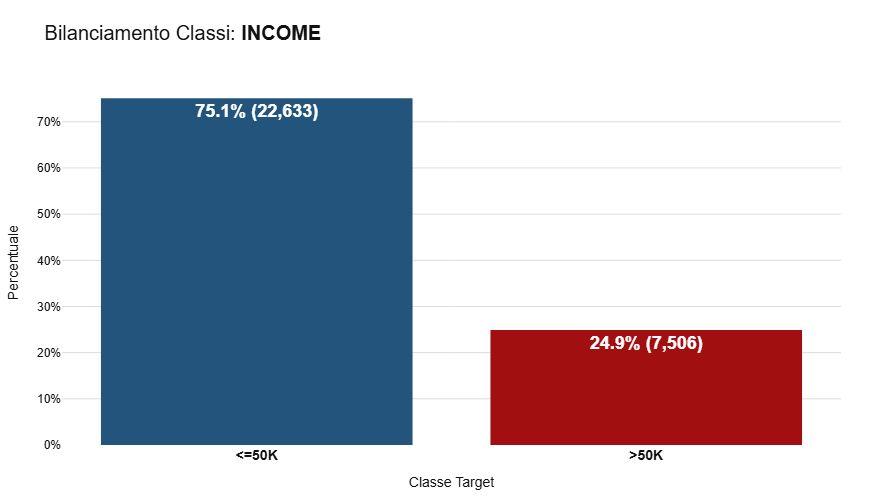
\includegraphics[width=0.75\linewidth]{figures/bilanciamenti_classe.png}
    \caption{\textbf{Distribuzione assoluta e relativa della variabile target} \texttt{income}. Il rapporto approssimativo è di 3:1.}
    \label{fig:bilanciamenti_classe.png}
\end{figure}

\noindent
Il rapporto di sbilanciamento pari a 3.15:1 ($\approx 24.1\% / 75.8\%$) ha importanti implicazioni:

\begin{enumerate}
    \item \textbf{Inadeguatezza dell'Accuracy:} Un classificatore dummy potrebbe predire sempre la classe maggioritaria, risultando però completamente inutile dal punto di vista predittivo.
    
    \item \textbf{Bias verso la classe maggioritaria:} Algoritmi di classificazione standard tendono a privilegiare il riconoscimento della classe dominante, specialmente se non opportunamente regolati. È pertanto necessario adottare metriche robuste (F1-score, ROC-AUC, Average Precision) e strategie di bilanciamento.
    
    \item \textbf{Insufficienza campionaria della classe minority:} Con soli 7.841 esempi positivi, il test set conterrà abbastanza osservazioni di classe minoritaria, fornendo stime di performance con varianza relativamente elevata. Sarà rilevante valutare intervalli di confidenza delle metriche.
    
    \item \textbf{Selezione della soglia decisionale:} La probabilità \textit{a priori} della classe minoritaria è pari a 0.241. Modelli di regressione logistica e probabilistici potranno essere calibrati per utilizzare questa soglia invece della soglia standard di 0.5, migliorando il compromesso Precision-Recall.
\end{enumerate}

\subsection{Analisi dei Valori Mancanti: Rilevamento, Quantificazione e Pattern}

\subsubsection{Decodifica e rilevamento dei placeholder}

Un primo controllo con i comandi pandas standard (\texttt{df.isnull().sum()}) non rivelava alcun valore \texttt{NaN}. Un'ispezione manuale di un sottoinsieme di record rivelò che i dati mancanti erano rappresentati dal token \texttt{?}.

La procedura di bonifica è stata la seguente:
\begin{enumerate}
    \item Sostituzione globale: \texttt{df.replace('?', np.nan, inplace=True)}
    \item Conversione esplicita a NaN per tutte le colonne categoriche
    \item Controllo post-conversione per validare l'assenza di artefatti
\end{enumerate}

\noindent
Tale approccio garantisce coerenza con i standard pandas e consente l'uso di metodi nativi per la gestione dei missing.

\subsubsection{Quantificazione per variabile}

La Tabella \ref{tab:missing} riporta il quadro completo della mancanza dati post-decodifica:

\begin{table}[H]
    \centering
    \begin{tabular}{lrr}
        \toprule
        \textbf{Variabile} & \textbf{Valori Mancanti} & \textbf{Percentuale (\%)} \\
        \midrule
        occupation & 1.843 & 5.66 \\
        workclass & 1.836 & 5.64 \\
        native.country & 583 & 1.79 \\
        \bottomrule
    \end{tabular}
    \caption{Riepilogo delle variabili con valori mancanti}
    \label{tab:missing}
\end{table}

\noindent
La mancanza è concentrata su tre sole variabili categoriche (\texttt{workclass}, \texttt{occupation}, \texttt{native.country}), tutte le variabili numeriche sono complete.

\subsubsection{Analisi strutturale della mancanza}

L'analisi della co-occorrenza della mancanza rivela un pattern non casuale (Figura \ref{fig:missing_heatmap}):

\begin{figure}[H]
    \centering
    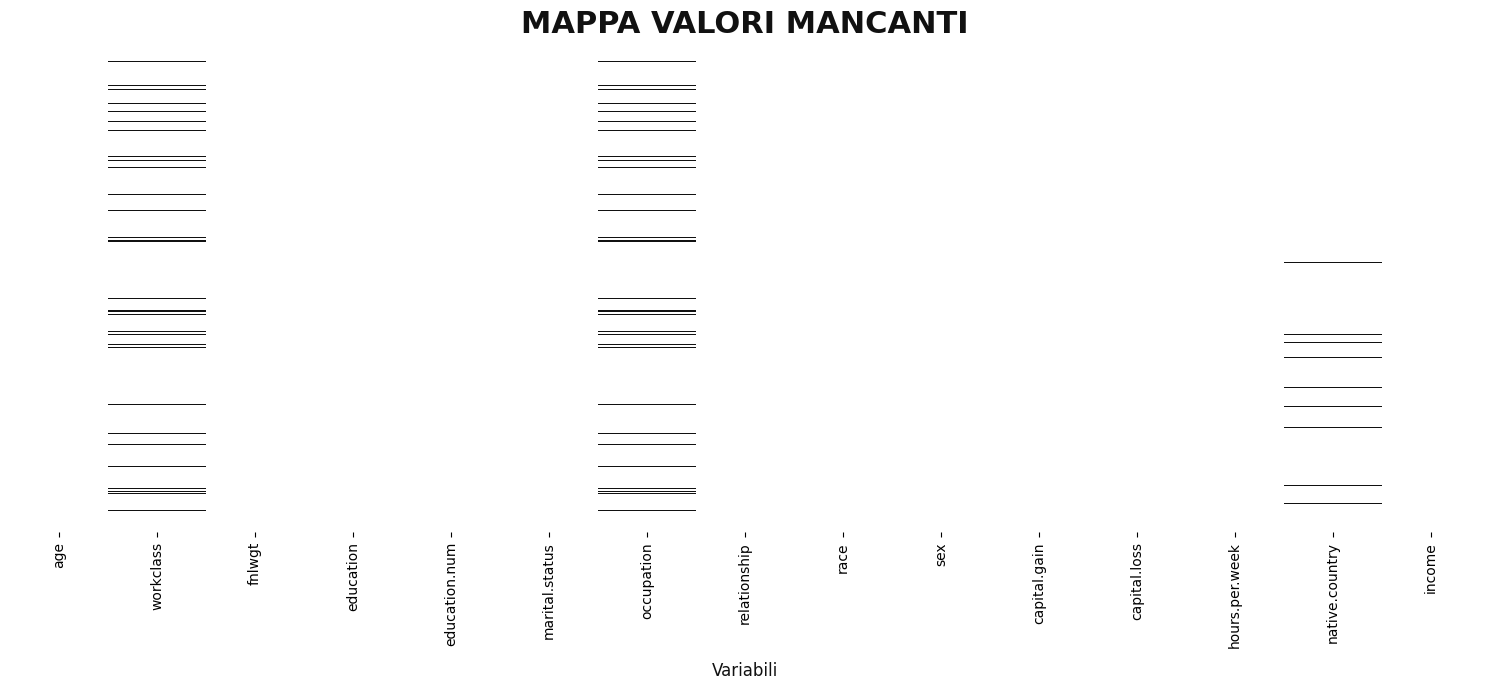
\includegraphics[width=\linewidth]{figures/mappa_valori_mancanti_2.png}
    \caption{\textbf{Heatmap della co-occorrenza dei valori mancanti.} La sovrapposizione visiva tra \texttt{workclass} e \texttt{occupation} suggerisce un pattern strutturale: individui privi di informazione su una variabile tendono a presentare un valore mancante anche nella seconda.}
    \label{fig:missing_heatmap}
\end{figure}

\noindent
Analisi quantitativa della co-occorrenza:
\begin{itemize}
    \item \textbf{Entrambi mancanti (workclass E occupation):} 1.836 osservazioni (di cui 27 estese anche a \texttt{native.country})
    \item \textbf{Solo occupation mancante:} 7 osservazioni
    \item \textbf{Solo native.country mancante:} 556 osservazioni
    \item \textbf{Dati completi:} 30.162 osservazioni (92.63\%)
\end{itemize}

\noindent
La concentrazione della mancanza congiunta (quasi il 100\% della mancanza in \texttt{workclass} si riflette in \texttt{occupation}) suggerisce un meccanismo \textit{Missing Not At Random} (MNAR), legato probabilmente a soggetti non occupati o categorie non censite, piuttosto che a un errore casuale di inserimento.

\subsubsection{Strategia di trattamento adottata}

Considerato che:
\begin{enumerate}
    \item La mancanza è strutturata e non casuale (MNAR)
    \item L'imputazione di variabili categoriche così specifiche potrebbe introdurre bias significativi nel modello predittivo
    \item Le variabili interessate sono solo 3 su 15, e la perdita totale è contenuta al \textbf{7.44\%}
    \item Il dataset rimane statisticamente robusto anche dopo la rimozione, conservando \textbf{30.139} osservazioni valide
\end{enumerate}

\noindent
Si è optato per la \textbf{listwise deletion}. Questa scelta garantisce la massima qualità del dato per le fasi successive di training, a fronte di una riduzione del campione considerata accettabile.

\begin{figure}[H]
    \centering
    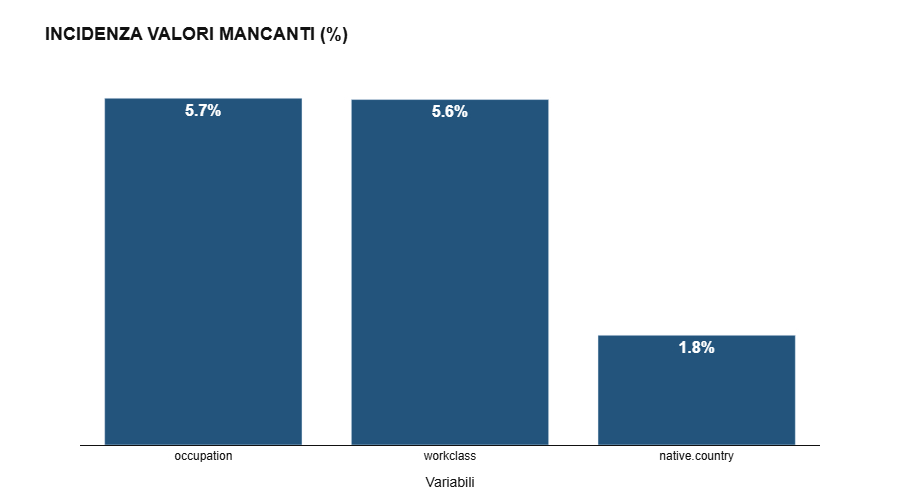
\includegraphics[width=\linewidth]{figures/incidenza_valori_mancanti.png}
    \caption{\textbf{Distribuzione percentuale dei valori mancanti per variabile.} Le variabili \texttt{occupation} (5.66\%), \texttt{workclass} (5.64\%) e \texttt{native.country} (1.79\%) rappresentano l'interezza dei dati mancanti nel dataset originale di 32.561 record.}
    \label{fig:missing_bar}
\end{figure}
\subsection{Analisi Descrittiva delle Variabili Categoriche}

\subsubsection{Strategia di analisi}

Per ciascuna variabile categorica è stata condotta un'analisi bidimensionale secondo il seguente protocollo:
\begin{enumerate}
    \item \textbf{Distribuzione marginale (assoluta e relativa):} frequenze e grafici a barre per visualizzare la cardinalità e il bilanciamento interno di ogni feature
    \item \textbf{Distribuzione condizionata rispetto al target:} suddivisione delle frequenze per classe di reddito, visualizzazione mediante barre affiancate o stacked
    \item \textbf{Proporzione della classe positiva per categoria:} calcolo della probabilità $P(income = >50K | \text{categoria})$ al fine di identificare categorie fortemente associate al reddito alto
\end{enumerate}

\noindent
Tale approccio consente di valutare sia la frequenza assoluta delle categorie (relevance per problemi di rarità) che la loro capacità discriminante, rilevante per la modellazione.

\subsubsection{Analisi di \texttt{workclass}}

\begin{figure}[H]
    \centering
    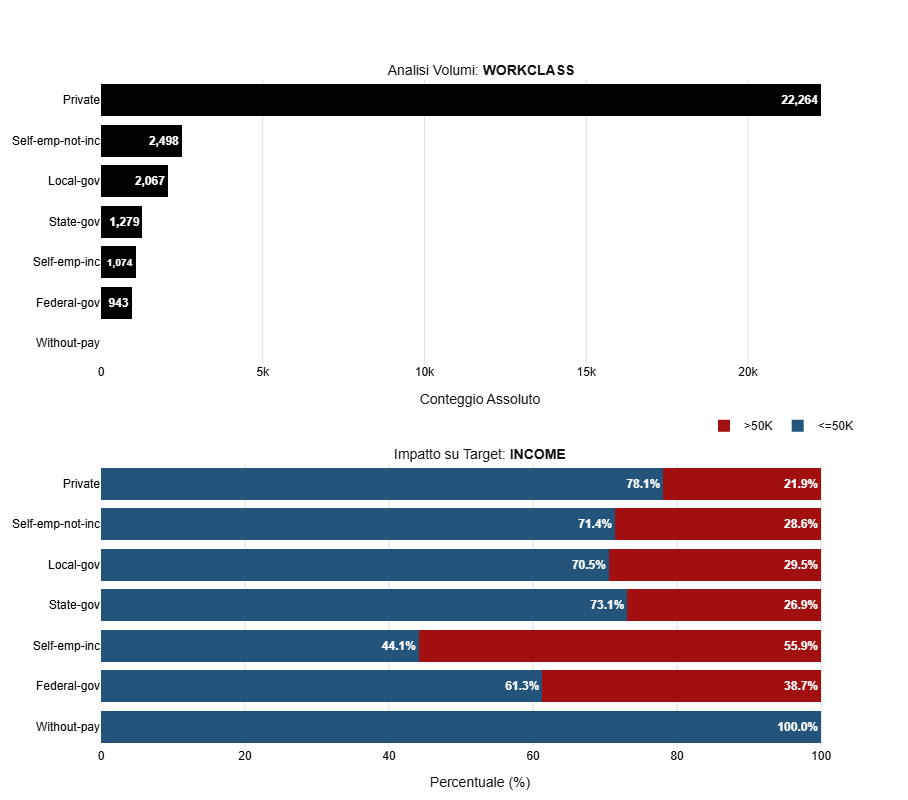
\includegraphics[width=0.9\linewidth]{figures/workclass1.png}
    \caption{\textbf{Analisi bivariata \texttt{workclass} vs \texttt{income}.} In alto: distribuzione assoluta delle categorie di classe lavorativa. In basso: proporzione della classe positiva per categoria, mostrando la capacità discriminante.}
    \label{fig:eda_workclass}
\end{figure}

\noindent
Osservazioni principali:
\begin{itemize}
    \item \textbf{Cardinalità:} 8 categorie, dominata da \textit{Private}
    \item \textbf{Discriminanza:} \textit{Self-emp-inc} (lavoratori autonomi incorporati) registra la probabilità più elevata di reddito $>50K$ (55.7\%), suggerendo una forte capacità predittiva
    \item \textbf{Categorie rare:} \textit{Without-pay e Never-worked} sono outlier, rappresentando categorie patologiche
\end{itemize}

\subsubsection{Analisi di \texttt{education}}

\begin{figure}[H]
    \centering
    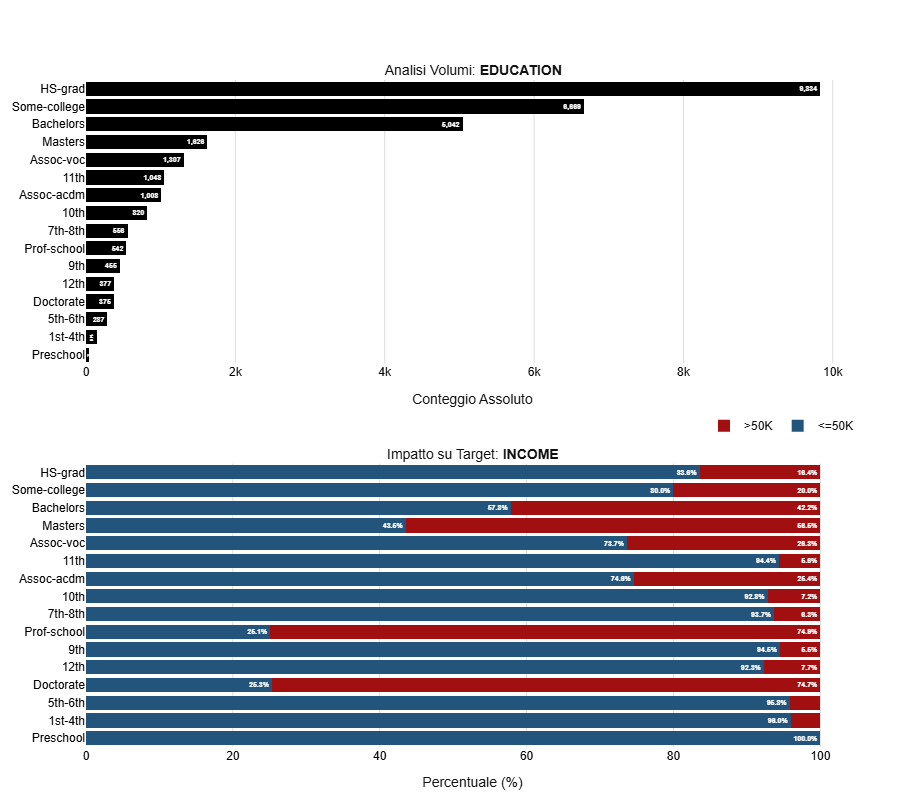
\includegraphics[width=\linewidth]{figures/education1.png}
    \caption{\textbf{Analisi bivariata \texttt{education} vs \texttt{income}.} La distribuzione mostra un ordinamento naturale (da Preschool a Doctorate).}
    \label{fig:eda_education}
\end{figure}

\noindent
Osservazioni principali:
\begin{itemize}
    \item \textbf{Ordinamento naturale:} A differenza di altre categoriche, education segue un ordinamento intrinseco (da meno a più istruzione)
    \item \textbf{Monotonicità della proporzione:} La probabilità $P(income = >50K)$ cresce in modo quasi monotono al crescere della scolarità: 0\% per Preschool, 74\% per Doctorate
    \item \textbf{Cardinalità:} 16 categorie, potenzialmente alta per alberi non ottimizzati
    \item \textbf{Alternativa numerica:} Esiste una variabile \texttt{education.num} che codifica numericamente questo ordinamento, suggerendo ridondanza informativa (da valutare in feature selection)
\end{itemize}

\subsubsection{Analisi di \texttt{marital.status}}

\begin{figure}[H]
    \centering
    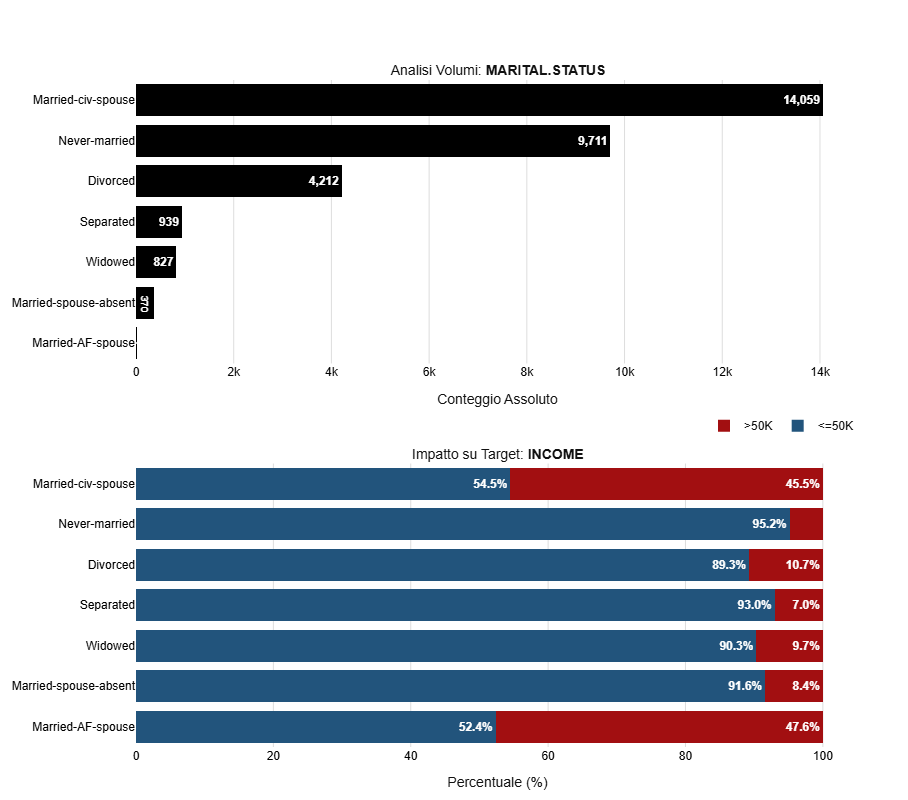
\includegraphics[width=0.9\linewidth]{figures/maritalstatus1.png}
    \caption{\textbf{Analisi bivariata \texttt{marital.status} vs \texttt{income}.} Lo stato civile emerge come uno dei predittori categorici più forti. Aver cessato il rapporto con il partner o non averne mai avuto mostra la bassa potenzialità a redditi $>50K$.}
    \label{fig:eda_marital}
\end{figure}

\noindent
Osservazioni principali:
\begin{itemize}
    \item \textbf{Discriminanza elevata:} Le categorie \textit{Married-civ-spouse} (44.7\%) e \textit{Married-AF-spouse} (43.5\%) mostrano probabilità di reddito alto quasi doppia rispetto alla media
    \item \textbf{Implicazione demografica:} Il matrimonio è storicamente associato a stabilità lavorativa e reddito più elevato, coerente con i dati
    \item \textbf{Sbilanciamento interno:} \textit{Never-married} è la seconda categoria più numerosa ma con la probabilità di reddito alto più bassa (4.6\%)
    \item \textbf{Cardinalità:} 7 categorie, gestibile
\end{itemize}

\subsubsection{Analisi di \texttt{occupation}}

\begin{figure}[H]
    \centering
    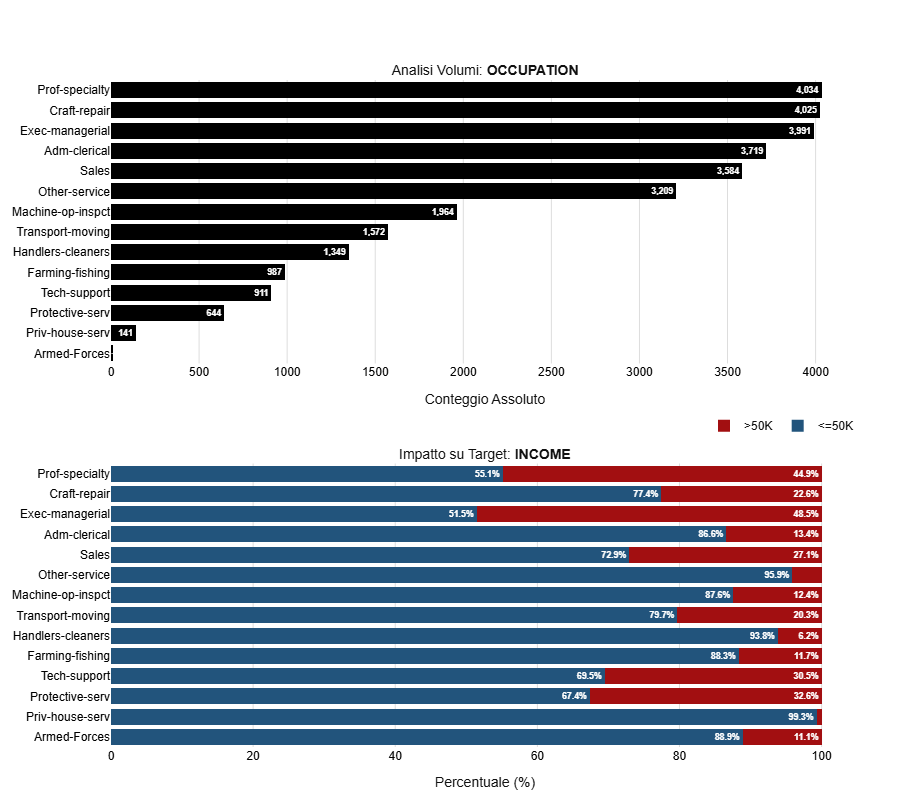
\includegraphics[width=\linewidth]{figures/occupation1.png}
    \caption{\textbf{Analisi bivariata \texttt{occupation} vs \texttt{income}.} Le professioni manageriali e specialistiche registrano le proporzioni più elevate di reddito alto.}
    \label{fig:eda_occupation}
\end{figure}

\noindent
Osservazioni principali:
\begin{itemize}
    \item \textbf{Discriminanza per ruolo:} \textit{Exec-managerial} (48.4\%) e \textit{Prof-specialty} (44.9\%) emergono come categorie ad alta capacità predittiva
    \item \textbf{Bimodalità implicita:} Le professioni si scindono chiaramente in "alte" (reddito > 50K probabile) e "basse" (es. \textit{Other-service} 4.2\%)
    \item \textbf{Cardinalità:} 14 categorie, ragionevolmente alta ma contenuta
\end{itemize}

\subsubsection{Analisi di \texttt{relationship}}

\begin{figure}[H]
    \centering
    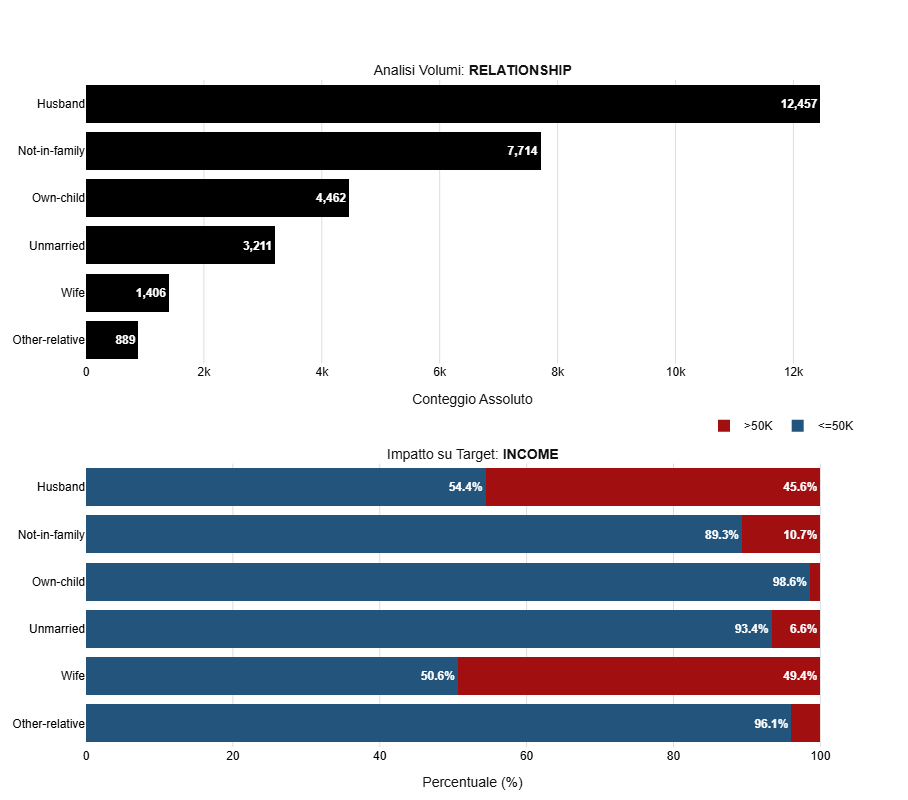
\includegraphics[width=\linewidth]{figures/relationship1.png}
    \caption{\textbf{Analisi bivariata \texttt{relationship} vs \texttt{income}.} Il ruolo familiare è strettamente correlato al target, con \textit{Husband} e \textit{Wife} dominanti nella classe positiva.}
    \label{fig:eda_relationship}
\end{figure}

\noindent
Osservazioni principali:
\begin{itemize}
    \item \textbf{Sovrapposizione con marital.status:} Esiste una forte relazione naturale con marital.status
    \item \textbf{Cardinalità bassa:} 6 categorie
\end{itemize}

\subsubsection{Analisi di \texttt{race}}

\begin{figure}[H]
    \centering
    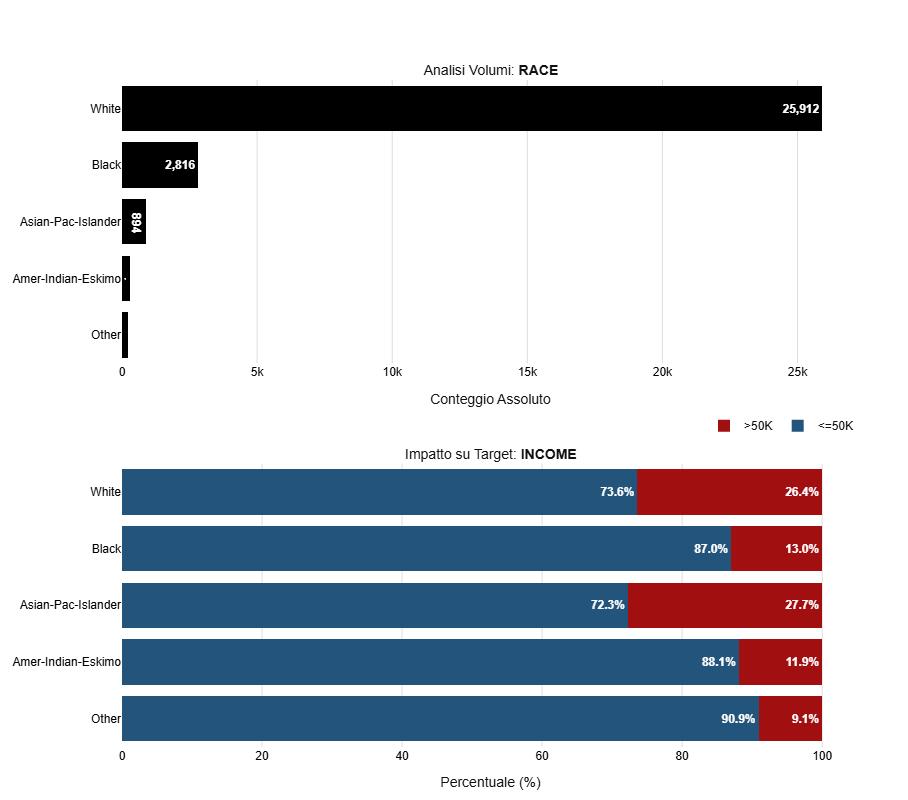
\includegraphics[width=0.9\linewidth]{figures/race1.png}
    \caption{\textbf{Analisi bivariata \texttt{race} vs \texttt{income}.} Emerge un marcato sbilanciamento campionario (> 86\% White) e disparità nelle proporzioni di reddito per gruppo etnico.}
    \label{fig:eda_race}
\end{figure}

\noindent
Osservazioni principali:
\begin{itemize}
    \item \textbf{Sbilanciamento campionario estremo:} White rappresenta il 86\% della popolazione, Asian-Pac-Islander circa il 3.0\%, altre categorie < 1 \%
    \item \textbf{Disparità reddituali:} Asian-Pac-Islander registra la proporzione più elevata di reddito alto (27.7\%), seguita da White (26.4\%)
    \item \textbf{Sensibilità etica:} La variabile race in contesti predittivi sensibili richiede cautela nell'interpretazione e nella comunicazione dei risultati
\end{itemize}

\subsubsection{Analisi di \texttt{sex}}

\begin{figure}[H]
    \centering
    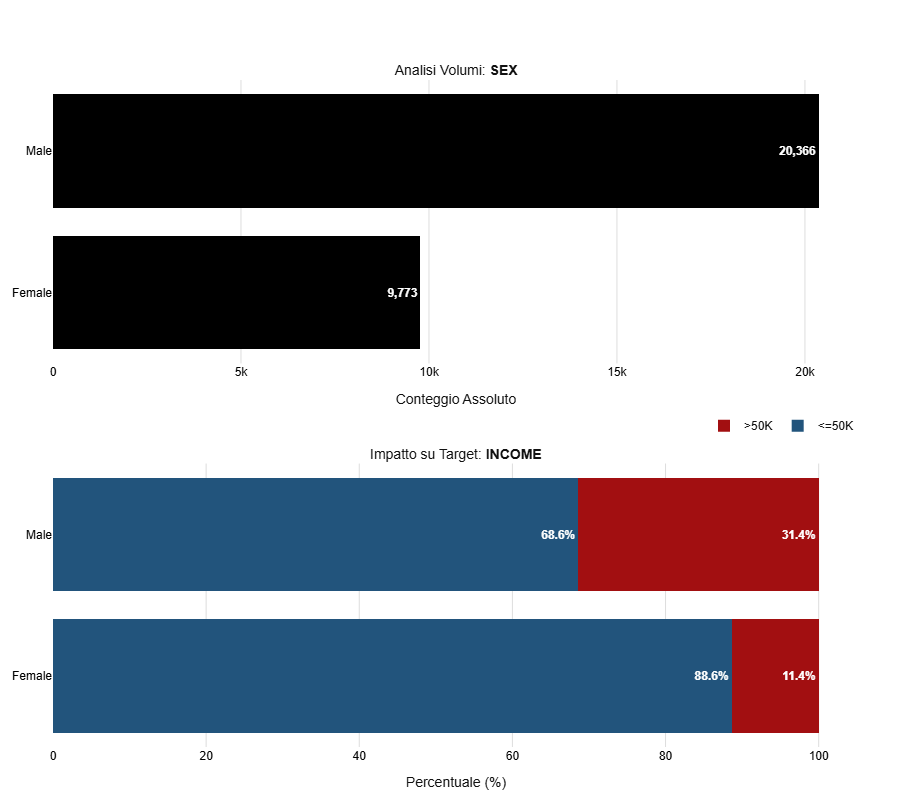
\includegraphics[width=\linewidth]{figures/sex1.png}
    \caption{\textbf{Analisi bivariata \texttt{sex} vs \texttt{income}.} Gap di genere marcato: il 31.4\% degli uomini ma solo 11.4\% delle donne raggiunge reddito > 50K nel dataset.}
    \label{fig:eda_sex}
\end{figure}

\noindent
Osservazioni principali:
\begin{itemize}
    \item \textbf{Gap reddituario:} Differenza proporzionale di 20 punti percentuali (31.4\% vs 11.4\%)
    \item \textbf{Cardinalità minima:} 2 categorie (possibilità di conversione binaria diretta per alcuni algoritmi)
    \item \textbf{Implicazione sociologica:} Il gap riflette disparità storiche nel mercato del lavoro, preservate nel dataset censuario
\end{itemize}

\subsubsection{Analisi di \texttt{native.country}}

\begin{figure}[H]
    \centering
    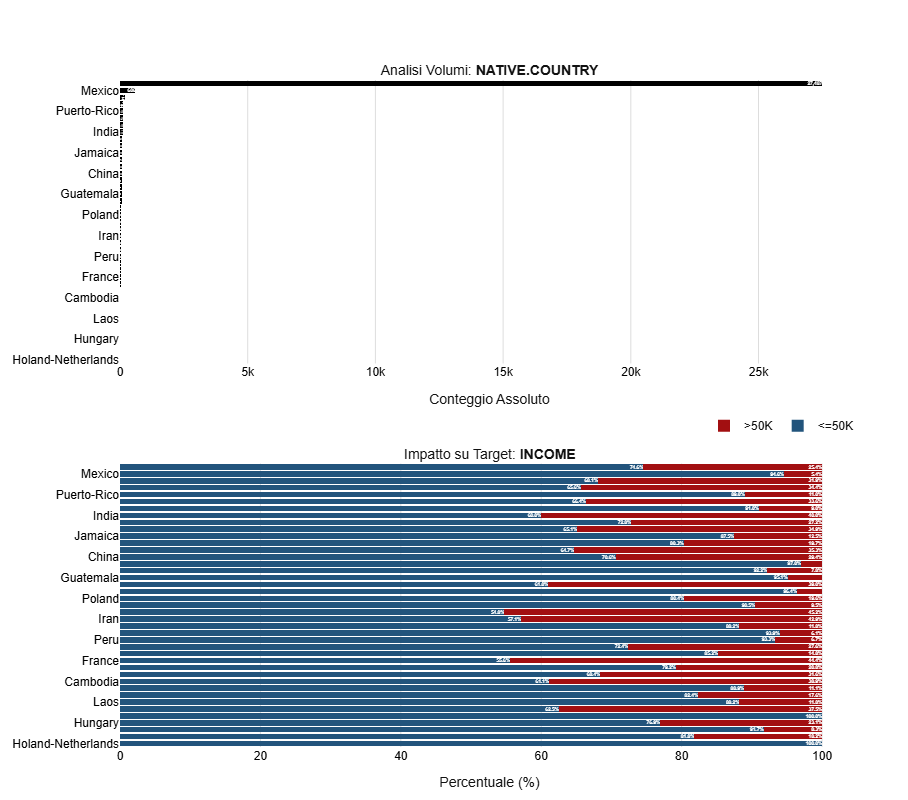
\includegraphics[width=\linewidth]{figures/nativecountry1.png}
    \caption{\textbf{Analisi bivariata \texttt{native.country} vs \texttt{income}.} Si osserva un'estrema polarizzazione verso gli \textit{United-States} (91.2\%), con una dispersione di micro-categorie per le restanti 40 nazioni.}
    \label{fig:eda_country}
\end{figure}

\noindent
Osservazioni principali:
\begin{itemize}
    \item \textbf{Dominanza statistica:} Gli \textit{United-States} rappresentano il \textbf{91.2\%} del campione (27.487 osservazioni) con un tasso di reddito elevato ($>50K$) del 25.4\%, valore che funge da baricentro per l'intero dataset.
    \item \textbf{Sparsità estrema:} Nonostante vi siano 41 valori unici, solo il \textbf{Mexico} (606 obs, 2.0\%) supera l'1\% di rappresentatività oltre agli USA. Paesi come \textit{Philippines} (0.6\%) e \textit{Germany} (0.4\%) mostrano frequenze troppo basse per garantire robustezza statistica individuale.
    \item \textbf{Eterogeneità del Target:} Si notano forti variazioni nel tasso di reddito tra le minoranze; ad esempio, \textit{Taiwan} (45.2\%) e \textit{Iran} (42.9\%) mostrano incidenze di reddito elevato molto superiori alla media, mentre \textit{Columbia} (3.6\%) e \textit{Dominican-Republic} (3.0\%) presentano valori minimi.
    \item \textbf{Implicazione di Feature Engineering:} L'alta cardinalità combinata con la presenza di categorie quasi nulle (es. \textit{Holand-Netherlands} con 1 sola osservazione) rende necessaria un'aggregazione in macro-aree geografiche o una binarizzazione ("USA" vs "Others") per prevenire l'overfitting e ridurre la dimensionalità dello spazio delle feature.
\end{itemize}


\subsection{Analisi Multivariata: Segmentazione per Genere}

Al fine di identificare potenziali bias demografici o differenze strutturali nella capacità discriminante delle \textit{feature}, è stata condotta un'analisi multivariata segmentando le variabili categoriche per la variabile \texttt{sex}. 

\begin{enumerate}[label=(\roman*)]
    \item \textbf{Obiettivo:} valutare come l'impatto delle singole variabili sul target vari tra uomini e donne, identificando categorie che potrebbero avere un peso predittivo differente nei due sottogruppi.
    \item \textbf{Metodologia visuale:} sono stati generati grafici a barre orizzontali normalizzati al 100\% (\textit{barnorm='percent'}). Questa scelta consente di confrontare direttamente le probabilità condizionate $P(income > 50K | feature, sex)$, eliminando l'effetto distorsivo dei volumi assoluti (essendo il campione maschile numericamente superiore).
\end{enumerate}

\begin{figure}[H]
    \centering
    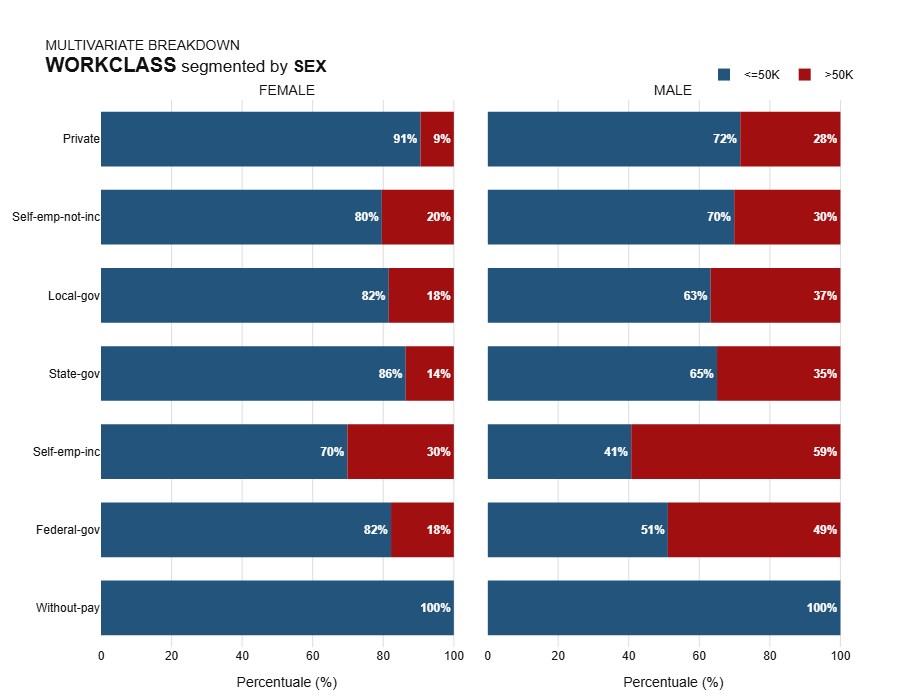
\includegraphics[width=\linewidth]{figures/worklass2.png} 
    \caption{\textbf{Analisi multivariata segmentata per sesso.} Il grafico mostra come il sesso femminile tende ad avere un reddito inferiore al 50K. Mentre solo in \texttt{self-emp-inc} gli uomini sono per il 59\% con redditi superiori a 50K.}
    \label{fig:worklass2.png}
\end{figure}

\begin{figure}[H]
    \centering
    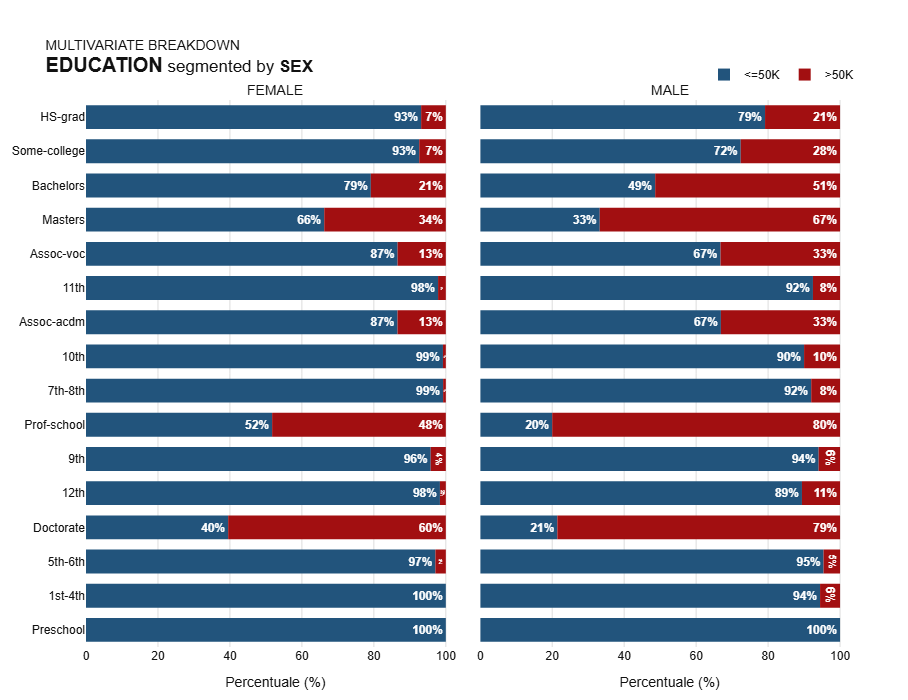
\includegraphics[width=\linewidth]{figures/education2.png} 
    \caption{\textbf{Analisi multivariata segmentata per sesso.} I generi mostrano che un alto livello di istruzione è associato a un reddito superiore, ma con differenze significative tra uomini e donne anche se seguono lo stesso andamento.}
    \label{fig:education2.png}
\end{figure}

\begin{figure}[H]
    \centering
    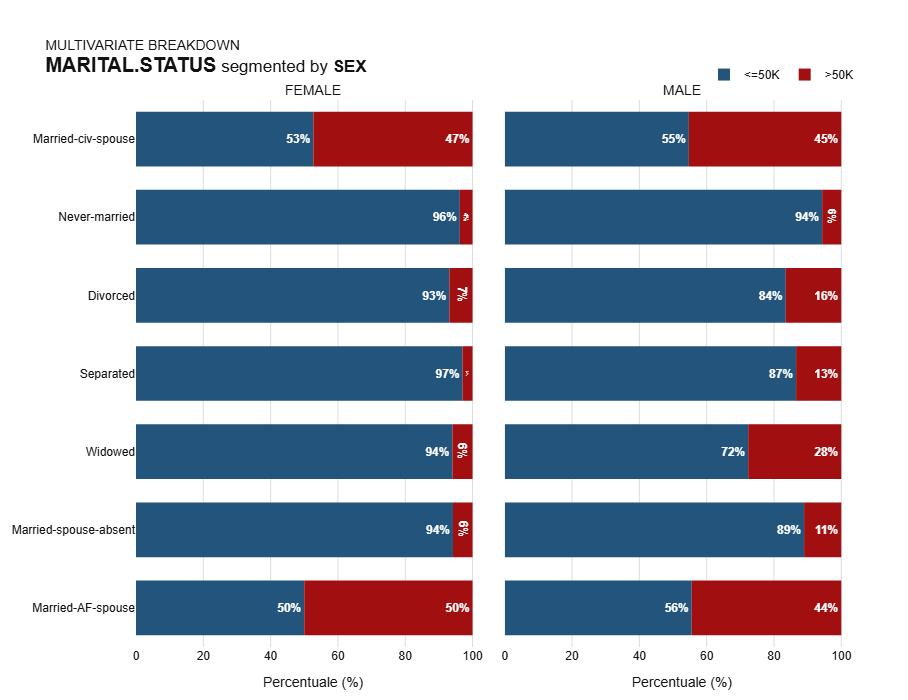
\includegraphics[width=\linewidth]{figures/maritalsstatus2.png} 
    \caption{\textbf{Analisi multivariata segmentata per sesso.} \texttt{marital-status} ci mostra che tra i generi nelle modalità "Married-civ-spouse" e "Married-AF-spouse" le donne hanno una percentuale di redditi superiori a 50K più bassa rispetto agli uomini. Per il resto gli uomini hanno sempre una percentuale più alta di redditi superiori a 50K.}
    \label{fig:aritalsstatus2.png}
\end{figure}

\begin{figure}[H]
    \centering
    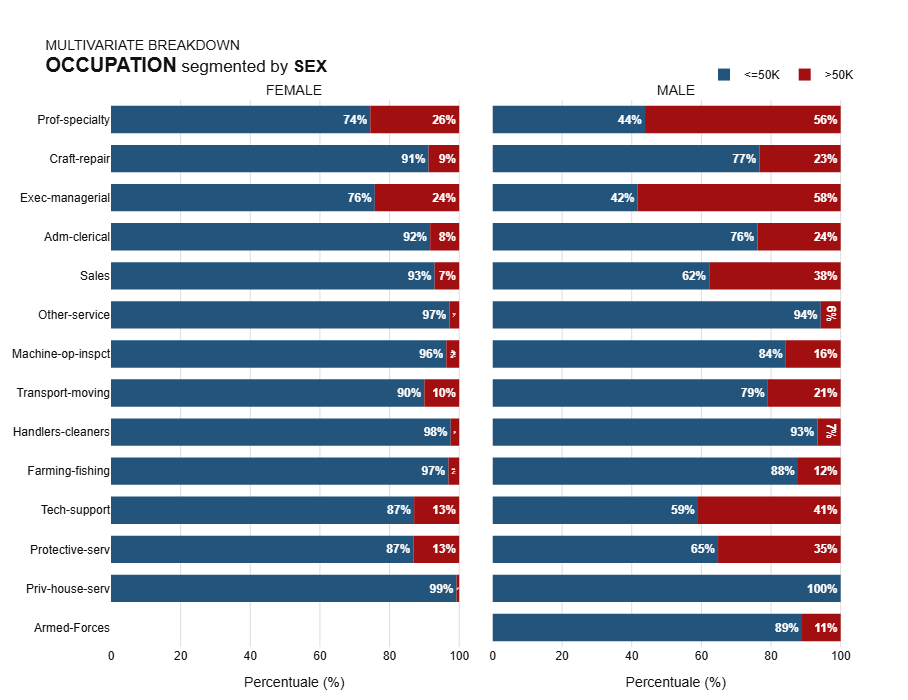
\includegraphics[width=\linewidth]{figures/occupation2.png} 
    \caption{\textbf{Analisi multivariata segmentata per sesso.} L'occupazione non è immune al gap di genere: in quasi tutte le categorie, gli uomini mostrano una proporzione più elevata di redditi > 50K rispetto alle donne.}
    \label{fig:occupation2.png}
\end{figure}

\begin{figure}[H]
    \centering
    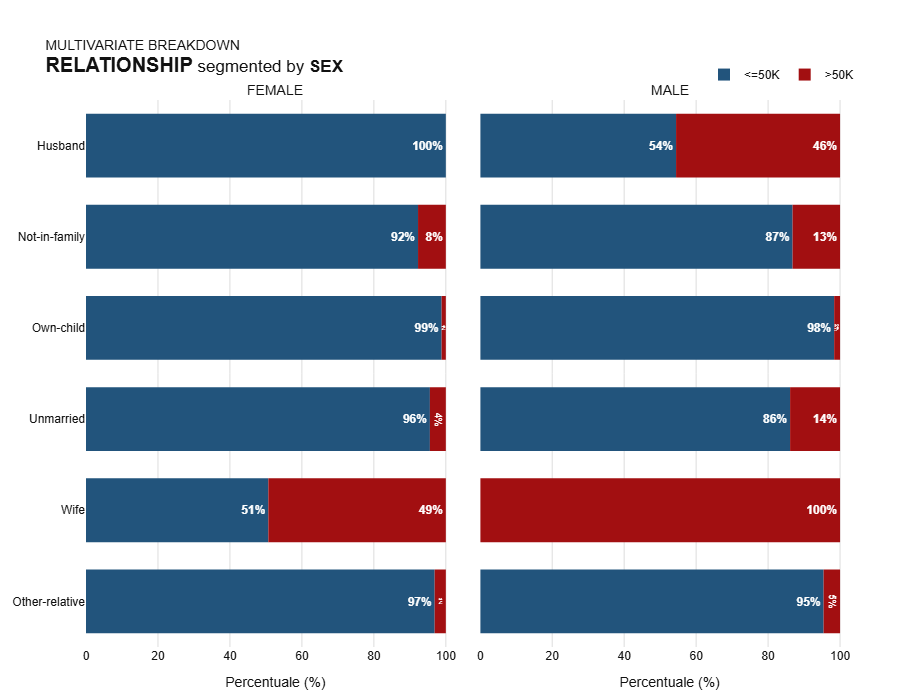
\includegraphics[width=\linewidth]{figures/relationship2.png} 
    \caption{\textbf{Analisi multivariata segmentata per sesso.} Il ruolo familiare mostra un pattern simile a marital.status, con gli uomini che tendono ad avere una maggiore proporzione di redditi elevati in quasi tutte le categorie, evidenziando un possibile effetto di interazione tra ruolo familiare e genere. Si evidenzia che le donne che sono "Wife" hanno una percentuale di redditi superiori a 50K più bassa rispetto agli uomini che sono "Husband".}
    \label{fig:relationship2.png}
\end{figure}

\begin{figure}[H]
    \centering
    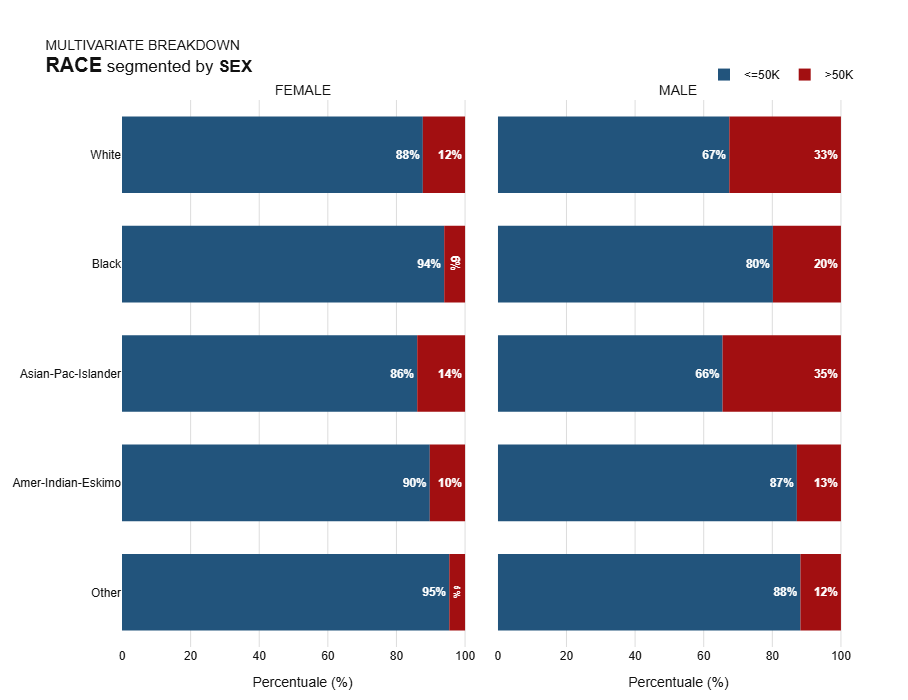
\includegraphics[width=\linewidth]{figures/race2.png} 
    \caption{\textbf{Analisi multivariata segmentata per sesso.} L'etnia mostra differenze di reddito tra i generi, con gli uomini che tendono ad avere una maggiore proporzione di redditi elevati rispetto alle donne in tutte le categorie etniche.}
    \label{fig:race2.png}
\end{figure}

\begin{figure}[H]
    \centering
    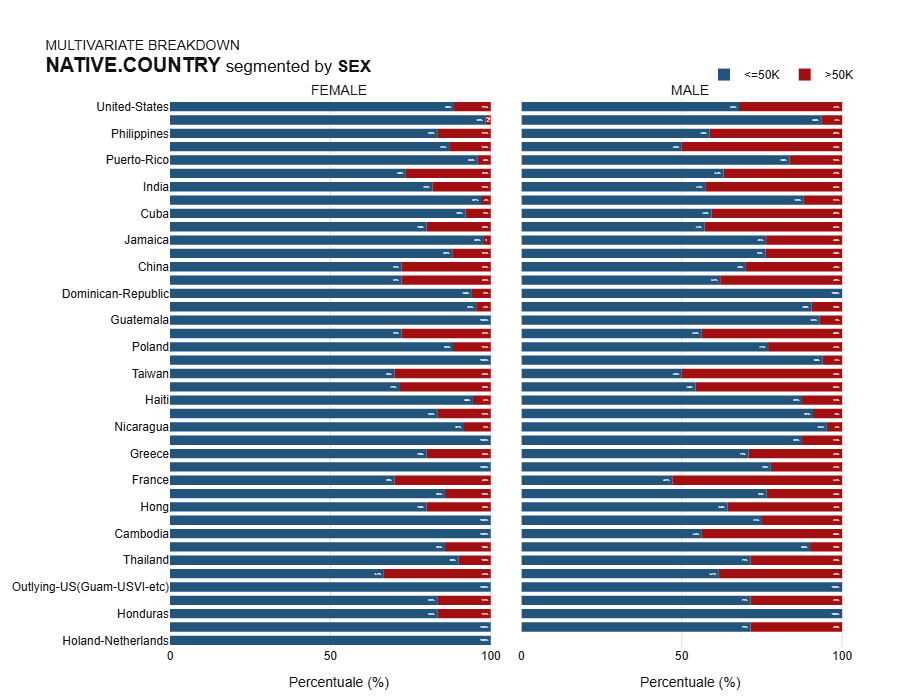
\includegraphics[width=\linewidth]{figures/nativecountry2.png} 
    \caption{\textbf{Analisi multivariata segmentata per sesso.} La nazionalità mostra un pattern di reddito più elevato per gli uomini rispetto alle donne in quasi tutte le categorie, con alcune eccezioni.}
    \label{fig:nativecountry2.png}
\end{figure}

\newpage

\subsection{Analisi Descrittiva delle Variabili Numeriche}

\subsubsection{Protocollo di analisi univariata}

Per ogni feature continua è stata condotta un'analisi distributzionale secondo:
\begin{enumerate}
    \item \textbf{Istogramma con kernel density estimate (KDE):} Visualizzazione della forma distributiva
    \item \textbf{Box plot:} Identificazione di outlier mediante IQR (intervallo interquartile)
    \item \textbf{Statistiche descrittive complete:} Media, mediana, std, min, max, quantili 25/75, Skewness, Kurtosis
    \item \textbf{Confronto condizionato sul target:} Overlay di distribuzioni per reddito $\leq 50K$ vs $> 50K$
\end{enumerate}

\noindent
Le metriche di forma distributiva sono critiche per valutare la necessità di trasformazioni (es. Box-Cox, log-transform) prima della modellazione con algoritmi sensibili alle code pesanti (es. regressione lineare, SVM).
% --- TABELLA RIEPILOGATIVA GENERALE ---
\subsubsection{Quadro Statistico Globale}

\begin{table}[H]
    \centering
    \caption{Statistiche descrittive globali delle variabili numeriche (N = 30.139)}
    \begin{adjustbox}{width=\textwidth,center}
    \begin{tabular}{lrrrrrrrrrrr}
        \toprule
        \textbf{Variabile} & \textbf{Media} & \textbf{Mediana} & \textbf{Moda} & \textbf{Dev. Std} & \textbf{CV} & \textbf{IQR} & \textbf{Min} & \textbf{Max} & \textbf{Skew} & \textbf{Kurt} \\
        \midrule
        age & 38.44 & 37.00 & 36.00 & 13.13 & 0.34 & 19.00 & 17.00 & 90.00 & 0.53 & -0.15 \\
        fnlwgt & 189,795 & 178,417 & 203,488 & 105,658 & 0.56 & 119,977 & 13,769 & 1,484,705 & 1.46 & 6.40 \\
        education.num & 10.12 & 10.00 & 9.00 & 2.55 & 0.25 & 4.00 & 1.00 & 16.00 & -0.30 & 0.64 \\
        capital.gain & 1,092.84 & 0.00 & 0.00 & 7,409.11 & 6.78 & 0.00 & 0.00 & 99,999 & 11.90 & 153.55 \\
        capital.loss & 88.44 & 0.00 & 0.00 & 404.45 & 4.57 & 0.00 & 0.00 & 4,356 & 4.52 & 19.49 \\
        hours.per.week & 40.93 & 40.00 & 40.00 & 11.98 & 0.29 & 5.00 & 1.00 & 99.00 & 0.33 & 3.17 \\
        \bottomrule
    \end{tabular}
    \end{adjustbox}
\end{table}

\vspace{1cm}

\newpage
% --- ANALISI DETTAGLIATA AGE ---
\subsubsection{Analisi di \texttt{age}}

\begin{table}[H]
    \centering
    \footnotesize
    \caption{Dettaglio \texttt{age} per gruppo di reddito e analisi del Delta}
    
    \textbf{Tabella A: Statistiche per Gruppo} \\
    \begin{tabular}{lrrrrrrrr}
        \toprule
        \textbf{income} & \textbf{Conteggio} & \textbf{Media} & \textbf{Mediana} & \textbf{Dev. Std} & \textbf{Min} & \textbf{Max} & \textbf{IQR} & \textbf{Skew} \\
        \midrule
        $\leq 50K$ & 22,633.00 & 36.61 & 34.00 & 13.46 & 17.00 & 90.00 & 19.00 & 0.74 \\
        $> 50K$ & 7,506.00 & 43.96 & 43.00 & 10.27 & 19.00 & 90.00 & 15.00 & 0.46 \\
        \bottomrule
    \end{tabular}

    \vspace{0.4cm}
    
    \textbf{Tabella B: Delta Report ($>50K$ vs $\leq 50K$)} \\
    \begin{tabular}{clrrrr}
        \toprule
        \textbf{ID} & \textbf{Metrica} & \textbf{$\leq 50K$ (Base)} & \textbf{$> 50K$ (Confronto)} & \textbf{Diff. Assoluta} & \textbf{Diff. \%} \\
        \midrule
        0 & Media & 36.61 & 43.96 & +7.35 & +20.07\% \\
        1 & Mediana & 34.00 & 43.00 & +9.00 & +26.47\% \\
        2 & Dev. Std & 13.46 & 10.27 & -3.19 & -23.70\% \\
        3 & IQR & 19.00 & 15.00 & -4.00 & -21.05\% \\
        \bottomrule
    \end{tabular}
\end{table}

\begin{figure}[H]
    \centering
    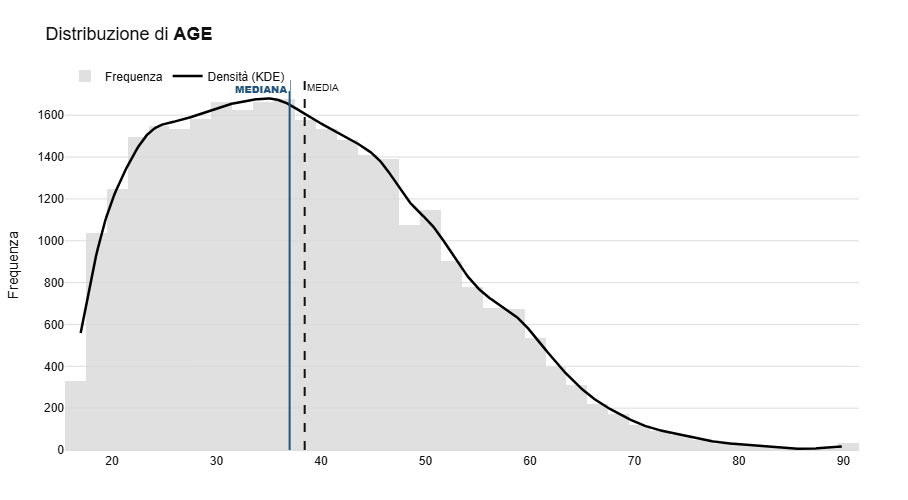
\includegraphics[width=1\linewidth]{figures/age1.png} % Sostituisci con il nome del tuo file immagine
    \caption{\textbf{Distribuzione di Age.} La discrepanza tra media e mediana evidenzia l'asimmetria positiva della distribuzione demografica.}
    \label{fig:uni_age}
\end{figure}

\begin{figure}[H]
    \centering
    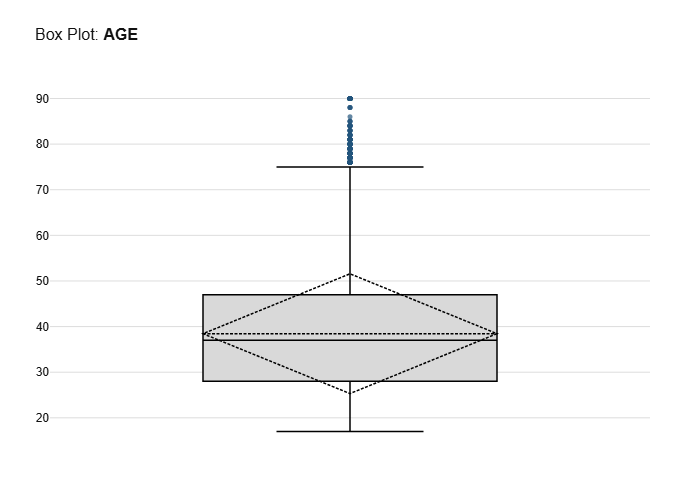
\includegraphics[width=0.8\linewidth]{figures/age_b.png} % Sostituisci con il nome del tuo file immagine
    \caption{\textbf{Boxplot di Age.} il 50\% dei valori si trova tra 30 e 50 anni.}
    \label{fig:age_b.png}
\end{figure}

\noindent
\textbf{Interpretazione:}
\begin{itemize}
    \item La distribuzione rimane approssimativamente normale con una leggera coda destra, tipica delle popolazioni lavorative.
    \item \textbf{Differenza bivariata su target:} Il delta tra le classi di reddito rimane significativo, suggerendo che l'anzianità favorisca redditi elevati fino alla soglia del pensionamento.
\end{itemize}

\newpage
% --- ANALISI DETTAGLIATA FNLWGT ---
\subsubsection{Analisi di \texttt{fnlwgt} (Final Weight)}

\begin{table}[H]
    \centering
    \footnotesize
    \caption{Dettaglio \texttt{fnlwgt} per gruppo di reddito e analisi del Delta}
    
    \textbf{Tabella A: Statistiche per Gruppo} \\
    \begin{tabular}{lrrrrrrrr}
        \toprule
        \textbf{income} & \textbf{Conteggio} & \textbf{Media} & \textbf{Mediana} & \textbf{Dev. Std} & \textbf{Min} & \textbf{Max} & \textbf{IQR} & \textbf{Skew} \\
        \midrule
        $\leq 50K$ & 22,633.00 & 190,342.15 & 179,508.00 & 106,575.12 & 13,769.00 & 1,484,705.00 & 122,097.00 & 1.48 \\
        $> 50K$ & 7,506.00 & 188,145.28 & 176,171.00 & 102,835.03 & 14,878.00 & 1,226,583.00 & 111,992.50 & 1.41 \\
        \bottomrule
    \end{tabular}

    \vspace{0.4cm}
    
    \textbf{Tabella B: Delta Report ($>50K$ vs $\leq 50K$)} \\
    \begin{tabular}{clrrrr}
        \toprule
        \textbf{ID} & \textbf{Metrica} & \textbf{$\leq 50K$ (Base)} & \textbf{$> 50K$ (Confronto)} & \textbf{Diff. Assoluta} & \textbf{Diff. \%} \\
        \midrule
        0 & Media & 190,342.15 & 188,145.28 & -2,196.87 & -1.15\% \\
        1 & Mediana & 179,508.00 & 176,171.00 & -3,337.00 & -1.86\% \\
        2 & Dev. Std & 106,575.12 & 102,835.03 & -3,740.08 & -3.51\% \\
        3 & IQR & 122,097.00 & 111,992.50 & -10,104.50 & -8.28\% \\
        \bottomrule
    \end{tabular}
\end{table}

\begin{figure}[H]
    \centering
    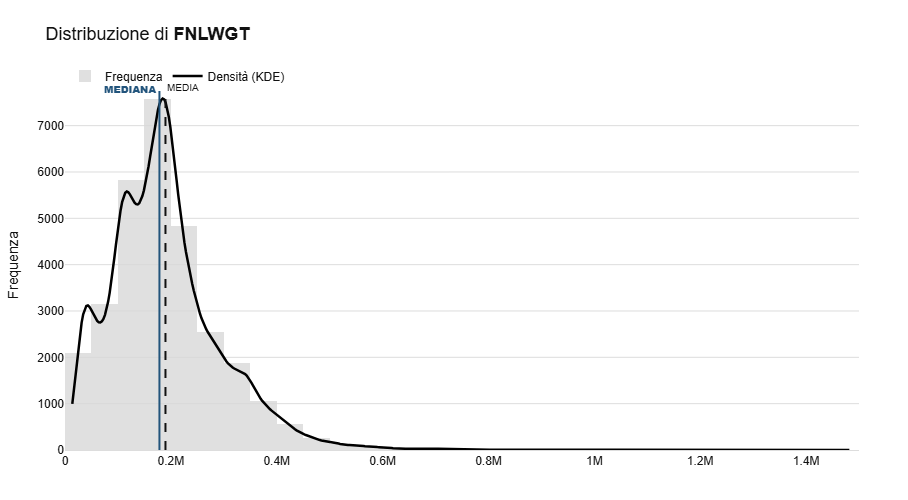
\includegraphics[width=1\linewidth]{figures/fnlwgt1.png}
    \caption{\textbf{Distribuzione di Final Weight.} La sovrapposizione quasi totale delle distribuzioni conferma l'assenza di potere predittivo.}
    \label{fig:uni_fnlwgt}
\end{figure}

\begin{figure}[H]
    \centering
    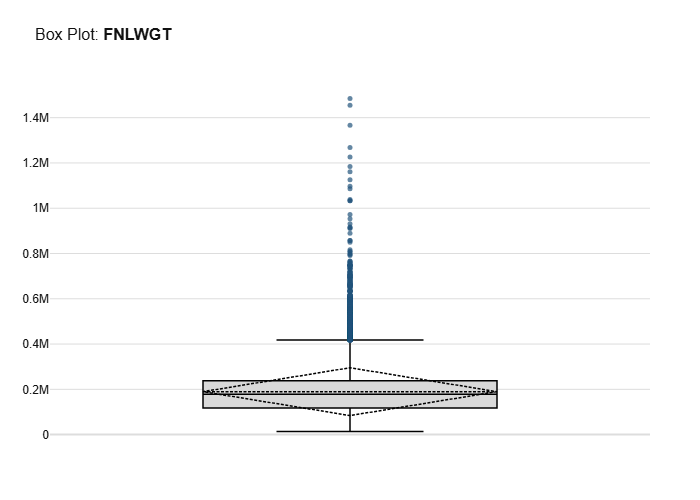
\includegraphics[width=0.8\linewidth]{figures/fnlwgt_b.png}
    \caption{\textbf{Boxplot di Final Weight.} valori estremi e outlier evidenti, con un range interquartile molto stretto.}
    \label{fig:fnlwgt_b.png}
\end{figure}

\noindent
\textbf{Interpretazione:}
\begin{itemize}
    \item La variabile mostra la sua natura di peso statistico amministrativo.
    \item L'alta kurtosis (+6.40) evidenzia la presenza di outlier estremi nella ponderazione demografica.
    \item \textbf{Decisione:} Si considera l'eventuale esclusione nelle fasi di addestramento dei modelli.
\end{itemize}

\newpage
% --- ANALISI DETTAGLIATA EDUCATION.NUM ---
\subsubsection{Analisi di \texttt{education.num}}

\begin{table}[H]
    \centering
    \footnotesize
    \caption{Dettaglio \texttt{education.num} per gruppo di reddito e analisi del Delta}
    
    \textbf{Tabella A: Statistiche per Gruppo} \\
    \begin{tabular}{lrrrrrrrr}
        \toprule
        \textbf{income} & \textbf{Conteggio} & \textbf{Media} & \textbf{Mediana} & \textbf{Dev. Std} & \textbf{Min} & \textbf{Max} & \textbf{IQR} & \textbf{Skew} \\
        \midrule
        $\leq 50K$ & 22,633.00 & 9.63 & 9.00 & 2.41 & 1.00 & 16.00 & 1.00 & -0.43 \\
        $> 50K$ & 7,506.00 & 11.61 & 12.00 & 2.37 & 2.00 & 16.00 & 3.00 & -0.30 \\
        \bottomrule
    \end{tabular}

    \vspace{0.4cm}
    
    \textbf{Tabella B: Delta Report ($>50K$ vs $\leq 50K$)} \\
    \begin{tabular}{clrrrr}
        \toprule
        \textbf{ID} & \textbf{Metrica} & \textbf{$\leq 50K$ (Base)} & \textbf{$> 50K$ (Confronto)} & \textbf{Diff. Assoluta} & \textbf{Diff. \%} \\
        \midrule
        0 & Media & 9.63 & 11.61 & +1.98 & +20.53\% \\
        1 & Mediana & 9.00 & 12.00 & +3.00 & +33.33\% \\
        2 & Dev. Std & 2.41 & 2.37 & -0.04 & -1.80\% \\
        3 & IQR & 1.00 & 3.00 & +2.00 & +200.00\% \\
        \bottomrule
    \end{tabular}
\end{table}

\begin{figure}[H]
    \centering
    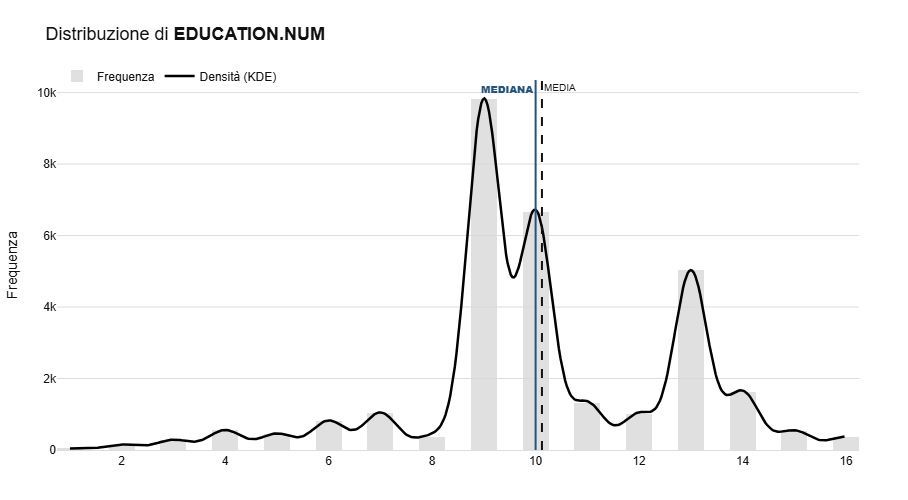
\includegraphics[width=1\linewidth]{figures/educationnum1.png}
    \caption{\textbf{Distribuzione di Education Num.} I picchi multipli riflettono la struttura a gradini dei cicli scolastici.}
    \label{fig:uni_edu}
\end{figure}

\begin{figure}[H]
    \centering
    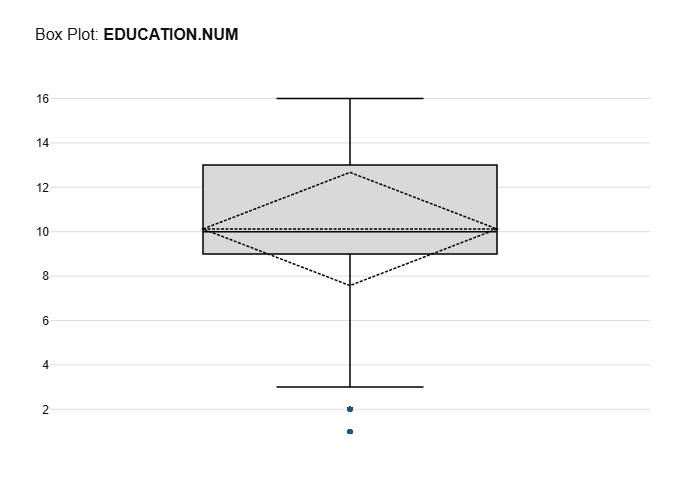
\includegraphics[width=0.8\linewidth]{figures/educationnum_b.png}
    \caption{\textbf{Boxplot di Education Num.} il 50\% dei casi è contenuto tra 9 e 13. Il grafico conferma una scarsa propensione in bassa istruzione della popolazione}
    \label{fig:edu_b.png}
\end{figure}

\noindent
\textbf{Interpretazione:}
\begin{itemize}
    \item La media leggermente superiore a 10 indica che il campione medio possiede un livello di istruzione superiore al diploma.
    \item L'asimmetria negativa (-0.30) riflette la concentrazione della popolazione verso livelli di istruzione medio-alti.
    \item \textbf{Relazione bivariata:} Si conferma come uno dei predittori più forti; la differenza del 33.33\% nella mediana (+3 anni di studio) è un segnale predittivo critico.
\end{itemize}

\newpage
% --- ANALISI DETTAGLIATA CAPITAL.GAIN ---
\subsubsection{Analisi di \texttt{capital.gain}}

\begin{table}[H]
    \centering
    \footnotesize
    \caption{Dettaglio \texttt{capital.gain} per gruppo di reddito e analisi del Delta}
    
    \textbf{Tabella A: Statistiche per Gruppo} \\
    \begin{tabular}{lrrrrrrrr}
        \toprule
        \textbf{income} & \textbf{Conteggio} & \textbf{Media} & \textbf{Mediana} & \textbf{Dev. Std} & \textbf{Min} & \textbf{Max} & \textbf{IQR} & \textbf{Skew} \\
        \midrule
        $\leq 50K$ & 22,633.00 & 149.03 & 0.00 & 936.82 & 0.00 & 41,310.00 & 0.00 & 17.41 \\
        $> 50K$ & 7,506.00 & 3,938.73 & 0.00 & 14,387.83 & 0.00 & 99,999.00 & 0.00 & 5.91 \\
        \bottomrule
    \end{tabular}

    \vspace{0.4cm}
    
    \textbf{Tabella B: Delta Report ($>50K$ vs $\leq 50K$)} \\
    \begin{tabular}{clrrrr}
        \toprule
        \textbf{ID} & \textbf{Metrica} & \textbf{$\leq 50K$ (Base)} & \textbf{$> 50K$ (Confronto)} & \textbf{Diff. Assoluta} & \textbf{Diff. \%} \\
        \midrule
        0 & Media & 149.03 & 3,938.73 & +3,789.70 & +2542.87\% \\
        1 & Mediana & 0.00 & 0.00 & +0.00 & +0.00\% \\
        2 & Dev. Std & 936.82 & 14,387.83 & +13,451.02 & +1435.82\% \\
        3 & IQR & 0.00 & 0.00 & +0.00 & +0.00\% \\
        \bottomrule
    \end{tabular}
\end{table}

\begin{figure}[H]
    \centering
    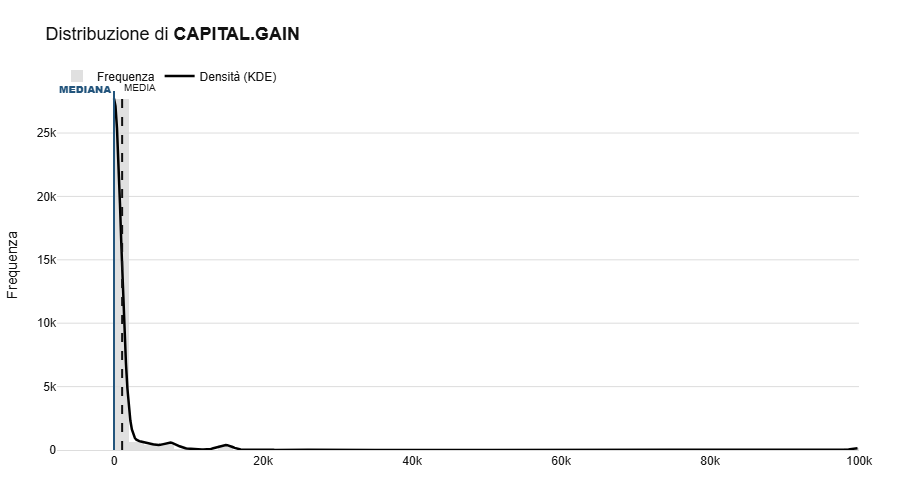
\includegraphics[width=1\linewidth]{figures/capitalgain1.png}
    \caption{\textbf{Distribuzione di Capital Gain.} La massa di osservazioni a zero domina completamente
la visualizzazione}
    \label{fig:uni_cap_gain}
\end{figure}

\begin{figure}[H]
    \centering
    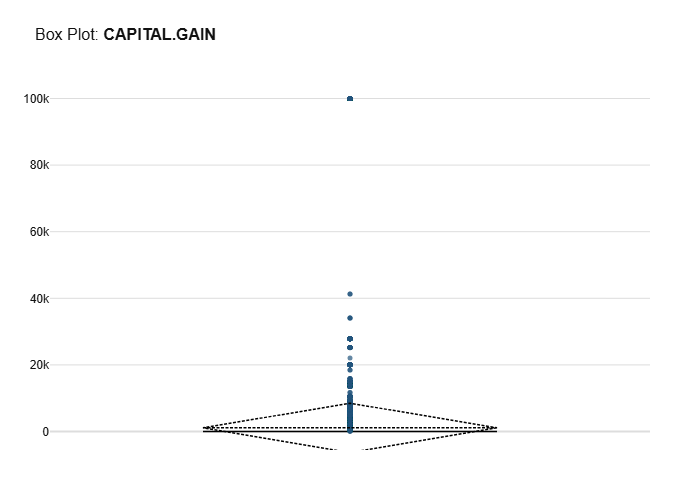
\includegraphics[width=0.8\linewidth]{figures/capitalgain_b.png}
    \caption{\textbf{Boxplot di Capital Gain.} Quasi la totalità dei valori è a zero. La presenza di outlier estremi è evidente con il max di 99,999.}
    \label{fig:capitalgain_b.png}
\end{figure}

\noindent
\textbf{Interpretazione:}
\begin{itemize}
    \item Persiste la caratteristica patologica di \textit{zero-inflation} (Mediana e Moda = 0).
    \item La kurtosis estrema (+153.55) indica una distribuzione quasi degenere su zero con eventi rarissimi di valore altissimo.
    \item \textbf{Trasformazione necessaria:} La differenza del +2542\% nella media tra le classi indica che, sebbene raro, il guadagno di capitale è quasi esclusivo della classe ad alto reddito.
\end{itemize}

\newpage
% --- ANALISI DETTAGLIATA CAPITAL.LOSS ---
\subsubsection{Analisi di \texttt{capital.loss}}

\begin{table}[H]
    \centering
    \footnotesize
    \caption{Dettaglio \texttt{capital.loss} per gruppo di reddito e analisi del Delta}
    
    \textbf{Tabella A: Statistiche per Gruppo} \\
    \begin{tabular}{lrrrrrrrr}
        \toprule
        \textbf{income} & \textbf{Conteggio} & \textbf{Media} & \textbf{Mediana} & \textbf{Dev. Std} & \textbf{Min} & \textbf{Max} & \textbf{IQR} & \textbf{Skew} \\
        \midrule
        $\leq 50K$ & 22,633.00 & 53.50 & 0.00 & 310.41 & 0.00 & 4,356.00 & 0.00 & 5.95 \\
        $> 50K$ & 7,506.00 & 193.80 & 0.00 & 592.90 & 0.00 & 3,683.00 & 0.00 & 2.80 \\
        \bottomrule
    \end{tabular}

    \vspace{0.4cm}
    
    \textbf{Tabella B: Delta Report ($>50K$ vs $\leq 50K$)} \\
    \begin{tabular}{clrrrr}
        \toprule
        \textbf{ID} & \textbf{Metrica} & \textbf{$\leq 50K$ (Base)} & \textbf{$> 50K$ (Confronto)} & \textbf{Diff. Assoluta} & \textbf{Diff. \%} \\
        \midrule
        0 & Media & 53.50 & 193.80 & +140.30 & +262.26\% \\
        1 & Mediana & 0.00 & 0.00 & +0.00 & +0.00\% \\
        2 & Dev. Std & 310.41 & 592.90 & +282.49 & +91.00\% \\
        3 & IQR & 0.00 & 0.00 & +0.00 & +0.00\% \\
        \bottomrule
    \end{tabular}
\end{table}

\begin{figure}[H]
    \centering
    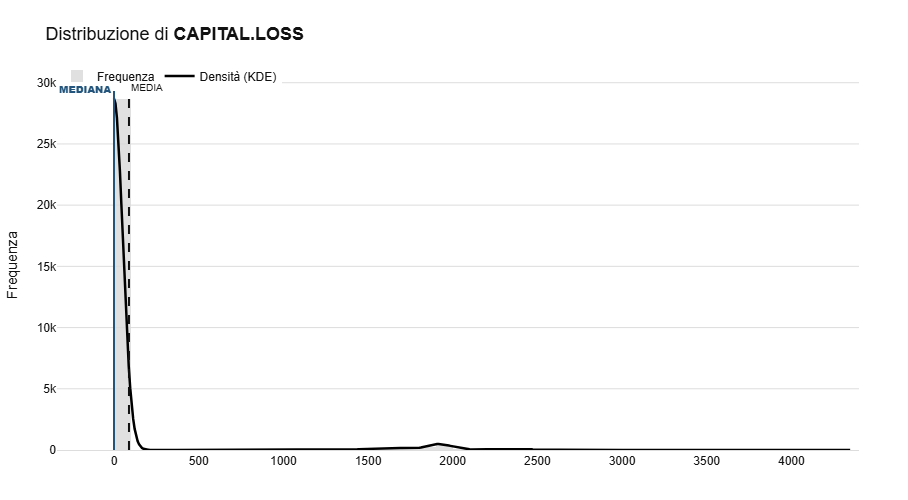
\includegraphics[width=1\linewidth]{figures/capitalloss1.png}
    \caption{\textbf{Distribuzione di Capital Loss.} Analogamente al gain, la variabile è dominata da zeri con una coda destra per investimenti falliti.}
    \label{fig:uni_cap_loss}
\end{figure}

\begin{figure}[H]
    \centering
    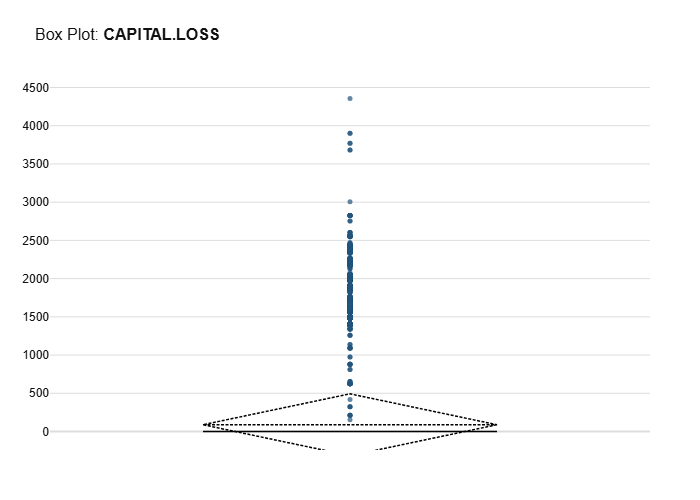
\includegraphics[width=1\linewidth]{figures/capitalloss_b.png}
    \caption{\textbf{Boxplot di Capital Loss.} Analogamente al gain, la variabile è dominata da zeri con una outlier.}
    \label{fig:capitalloss_b.png}
\end{figure}

\noindent
\textbf{Interpretazione:}
\begin{itemize}
    \item Comportamento analogo a \texttt{capital.gain}, con una prevalenza massiccia di zeri.
    \item \textbf{Implicazione:} La variabile è sparsa ma informativa; la differenza del 262\% nella media suggerisce che chi possiede asset finanziari (e subisce perdite) appartiene più frequentemente alla classe $>50K$.
\end{itemize}

\newpage
% --- ANALISI DETTAGLIATA HOURS.PER.WEEK ---
\subsubsection{Analisi di \texttt{hours.per.week}}

\begin{table}[H]
    \centering
    \footnotesize
    \caption{Dettaglio \texttt{hours.per.week} per gruppo di reddito e analisi del Delta}
    
    \textbf{Tabella A: Statistiche per Gruppo} \\
    \begin{tabular}{lrrrrrrrr}
        \toprule
        \textbf{income} & \textbf{Conteggio} & \textbf{Media} & \textbf{Mediana} & \textbf{Dev. Std} & \textbf{Min} & \textbf{Max} & \textbf{IQR} & \textbf{Skew} \\
        \midrule
        $\leq 50K$ & 22,633.00 & 39.35 & 40.00 & 11.95 & 1.00 & 99.00 & 2.00 & 0.30 \\
        $> 50K$ & 7,506.00 & 45.71 & 40.00 & 10.74 & 1.00 & 99.00 & 10.00 & 0.85 \\
        \bottomrule
    \end{tabular}

    \vspace{0.4cm}
    
    \textbf{Tabella B: Delta Report ($>50K$ vs $\leq 50K$)} \\
    \begin{tabular}{clrrrr}
        \toprule
        \textbf{ID} & \textbf{Metrica} & \textbf{$\leq 50K$ (Base)} & \textbf{$> 50K$ (Confronto)} & \textbf{Diff. Assoluta} & \textbf{Diff. \%} \\
        \midrule
        0 & Media & 39.35 & 45.71 & +6.36 & +16.15\% \\
        1 & Mediana & 40.00 & 40.00 & +0.00 & +0.00\% \\
        2 & Dev. Std & 11.95 & 10.74 & -1.21 & -10.13\% \\
        3 & IQR & 2.00 & 10.00 & +8.00 & +400.00\% \\
        \bottomrule
    \end{tabular}
\end{table}

\begin{figure}[H]
    \centering
    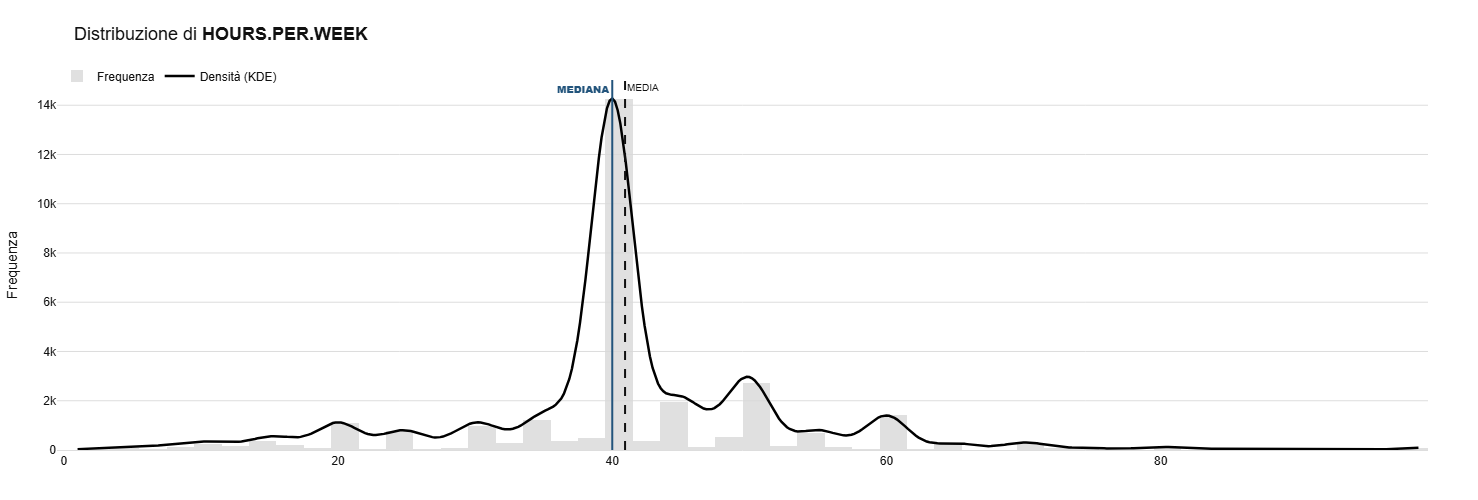
\includegraphics[width=1\linewidth]{figures/hoursperweek1.png}
    \caption{\textbf{Distribuzione di Hours per Week.} Si nota una concentrazione estrema sulla moda di 40 ore per entrambe le classi.}
    \label{fig:uni_hours}
\end{figure}

\begin{figure}[H]
    \centering
    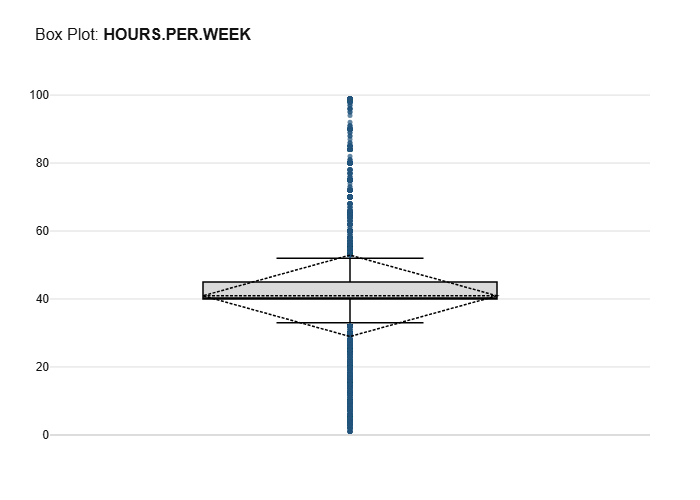
\includegraphics[width=0.8\linewidth]{figures/hoursperweek_b.png}
    \caption{\textbf{Boxplot di Hours per Week.} Il grafico mostra una bassa dispersione dei valori, si concentrano attorno dalle 40 ore settimanali. Si notano diversi outlier}
    \label{fig:hoursperweek_b.png}
\end{figure}

\noindent
\textbf{Interpretazione:}
\begin{itemize}
    \item La media di 45.71 ore per la classe $>50K$ rispetto alle 39.35 della classe base suggerisce la correlazione tra impegno orario e reddito.
    \item L'esplosione dell'IQR (+400\%) nella classe superiore indica una maggiore variabilità: i redditi alti lavorano o le canoniche 40 ore o significativamente di più (code pesanti).
    \item \textbf{Stabilità:} È la variabile continua più regolare del dataset, con una forte concentrazione sulla "settimana lavorativa standard".
\end{itemize}

\subsection{Analisi Bivariata: Boxplot e Pairplot}

\begin{figure}[H]
    \centering
    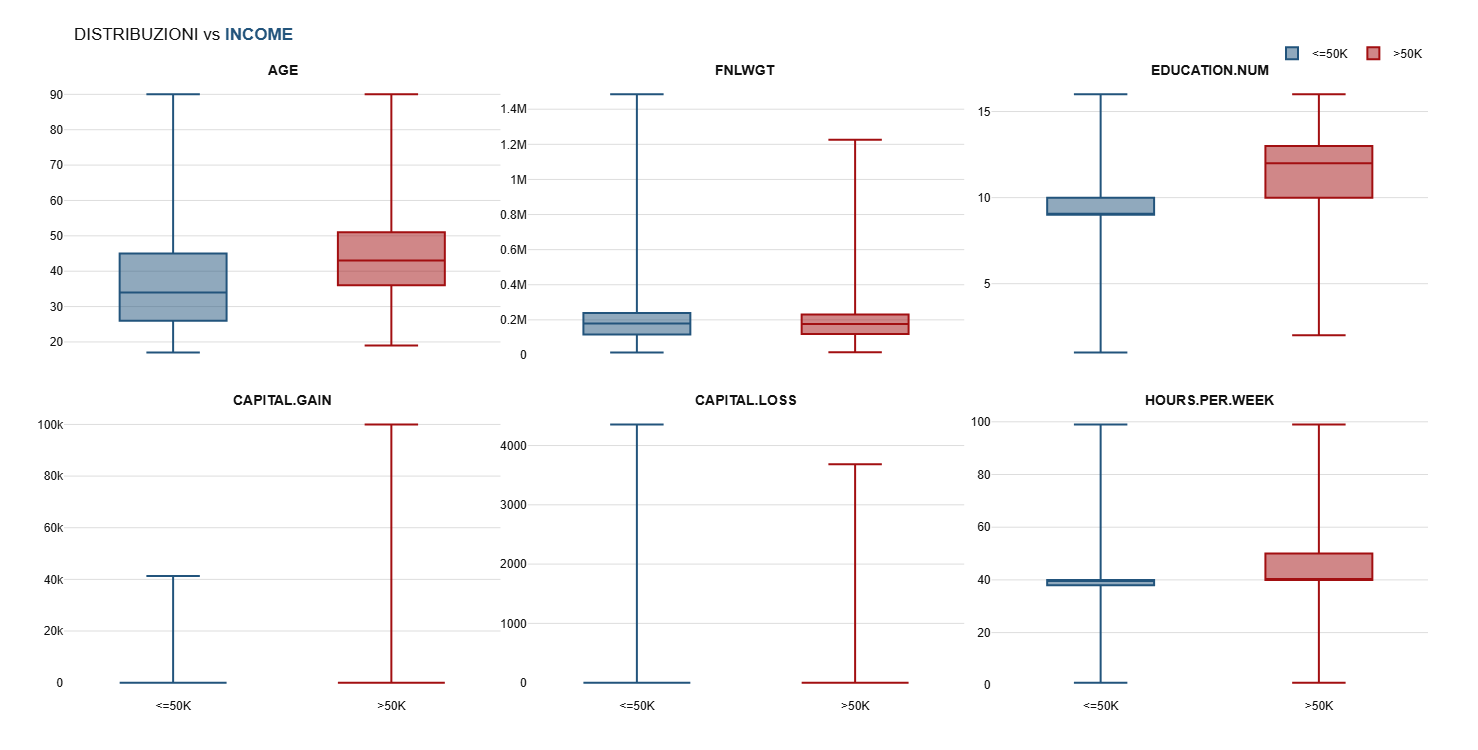
\includegraphics[width=1\linewidth]{figures/boxplot_confornti.png}
    \caption{\textbf{Comparazione dei boxplot delle categorie numeriche per classe.} La differenza più marcata si osserva in \texttt{education.num}, mentre \texttt{fnlwgt} mostra una sovrapposizione quasi totale.}
    \label{fig:boxplot_confronti.png}
\end{figure}

\begin{figure}[H]
    \centering
    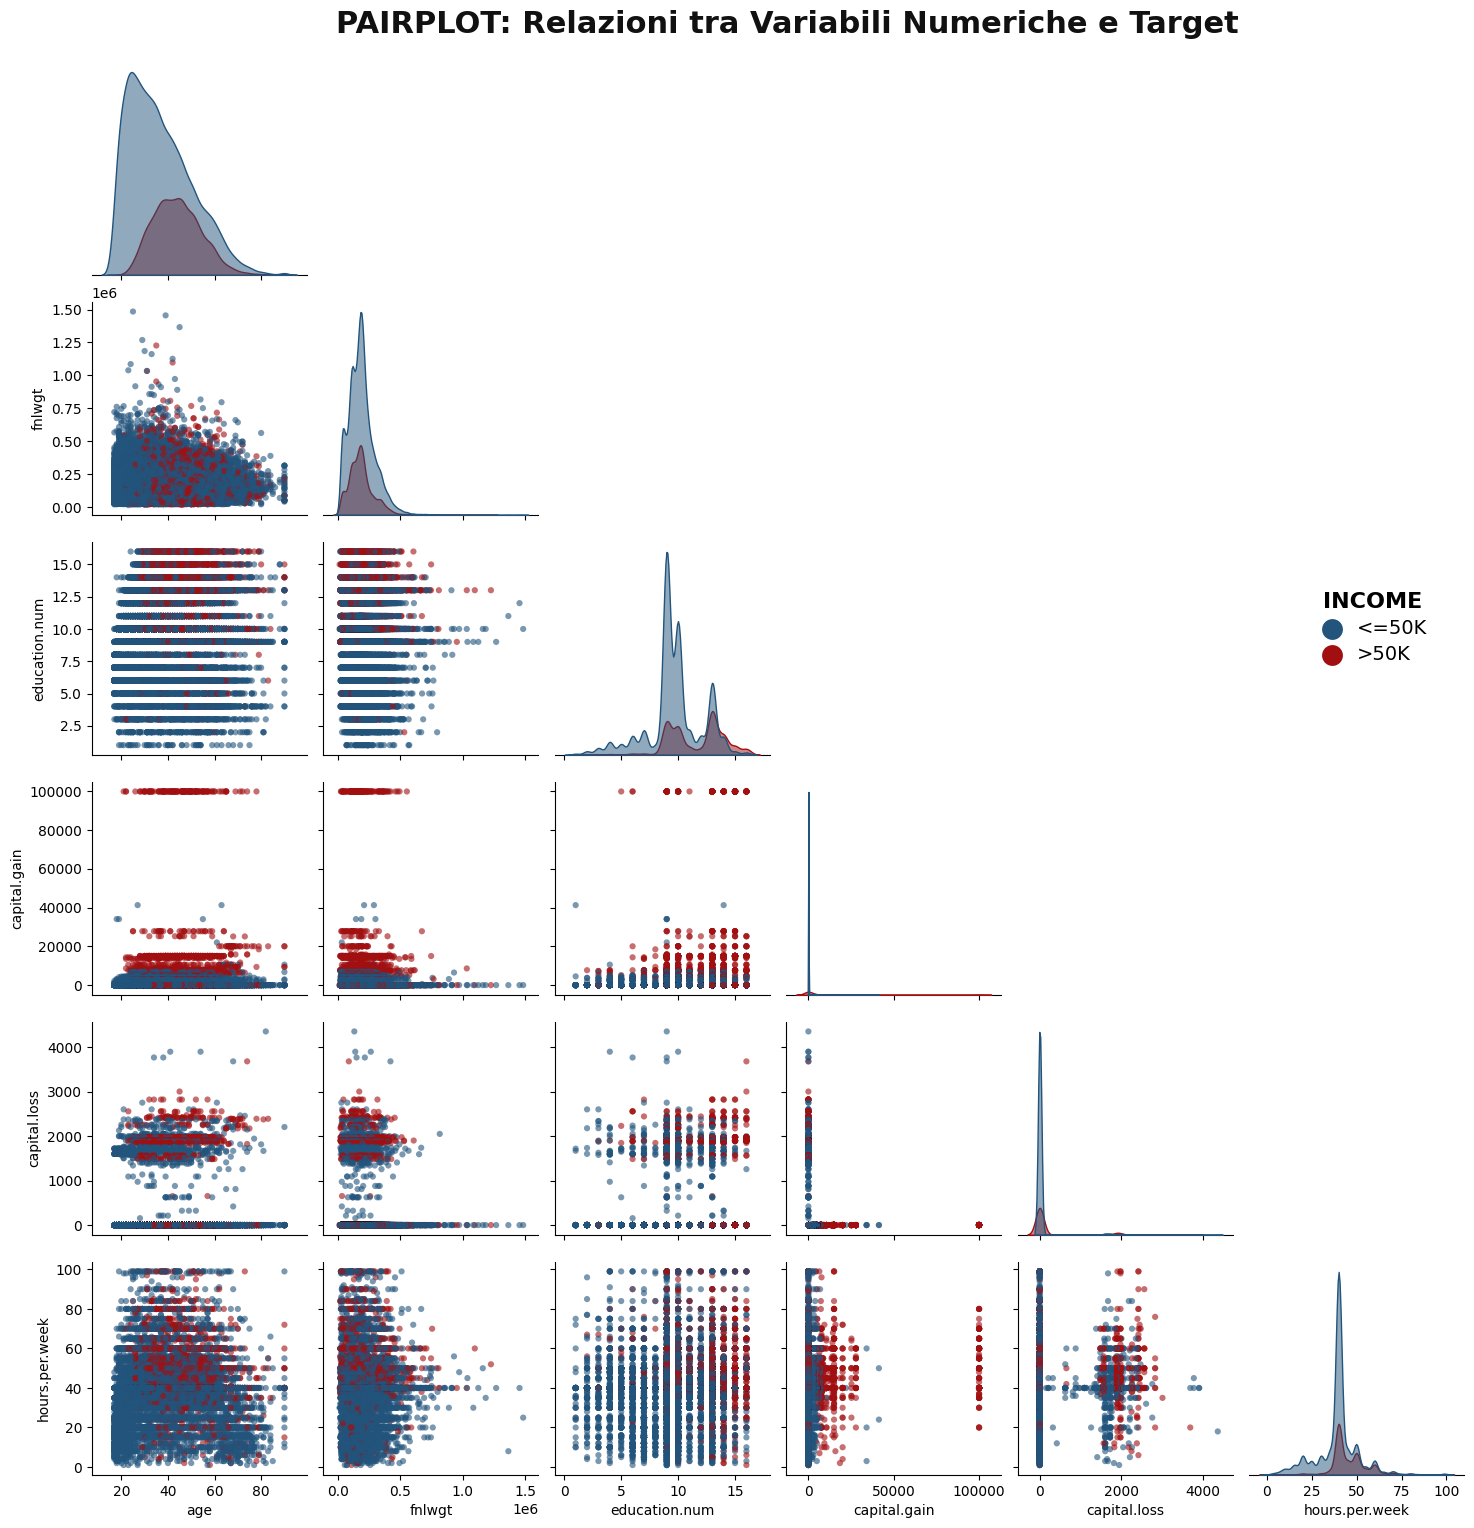
\includegraphics[width=1.01\linewidth]{figures/pairplot.png}
    \caption{\textbf{Pairplot.}}
    \label{fig:pairplot.png}
\end{figure}

\newpage
\subsection{Analisi delle Correlazioni tra Feature Numeriche}

\begin{figure}[H]
    \centering
    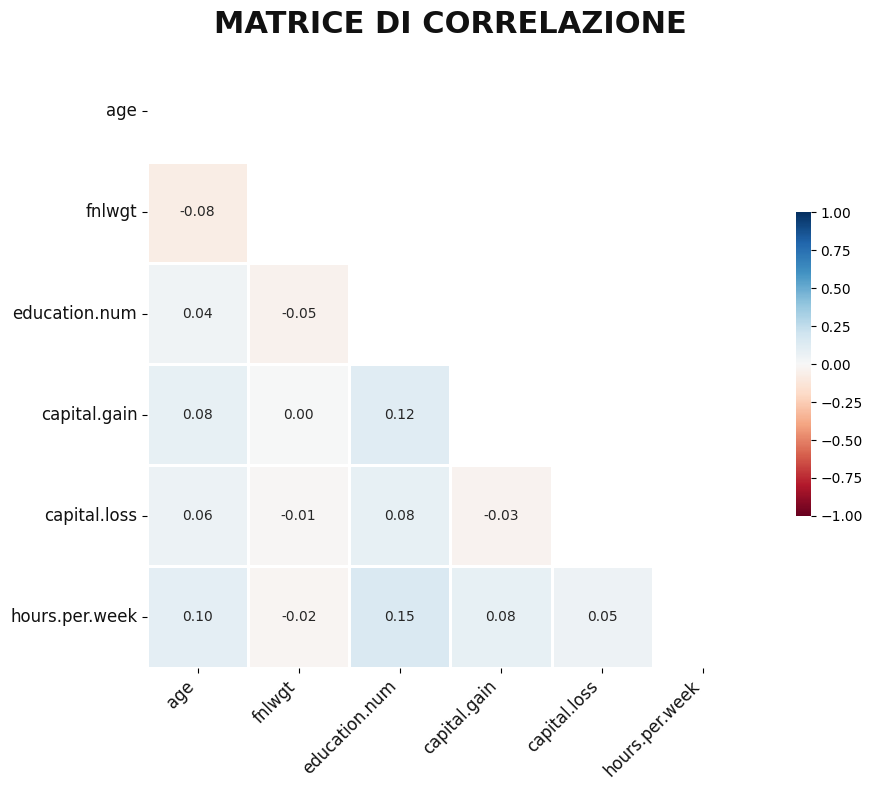
\includegraphics[width=0.8\linewidth]{figures/matrice_correlazione.png}
    \caption{\textbf{Matrice di Correlazione di Pearson.} I valori ridotti (max $r=0.15$) evidenziano un'assenza di multicollinearità e una forte indipendenza lineare tra le feature.}
    \label{fig:matrice_correlazione.png}
\end{figure}

Al fine di identificare potenziali ridondanze informative e valutare il rischio di multicollinearità, è stata analizzata la matrice di correlazione per le variabili numeriche.
I risultati evidenziano uno scenario di forte indipendenza lineare tra i predittori. Come si evince dai dati, non emerge alcun cluster di variabili fortemente correlate. Nello specifico:

\begin{itemize}
    \item \textbf{Assenza di Multicollinearità:} Il coefficiente massimo registrato nell'intera matrice è pari a $r = 0.15$. Tale valore è inferiore alle soglie di allarme tipicamente considerate critiche in letteratura ($|r| > 0.85$), garantendo che nessuna feature numerica sia una combinazione lineare delle altre.
    
    \item \textbf{Relazioni Deboli ma Interpretabili:} Anche le associazioni logicamente attese risultano deboli. Ad esempio, la correlazione tra (\texttt{education.num}) e (\texttt{capital.gain}) si attesta su un modesto $r = 0.12$. Questo suggerisce che, sebbene esista una lieve tendenza positiva, le due variabili catturano aspetti diversi del profilo socio-economico dell'individuo.
    
    \item \textbf{Neutralità del Peso Campionario:} La variabile \texttt{fnlwgt} mostra correlazioni quasi nulle con tutte le altre feature (valori compresi tra $-0.08$ e $0.00$). Ciò conferma empiricamente che il peso statistico assegnato dal censimento è ortogonale alle caratteristiche demografiche del soggetto.
\end{itemize}

\noindent
\textbf{Implicazioni per la modellazione:} 
Data l'assenza di ridondanza informativa tra le variabili, non si ritiene necessario applicare tecniche di feature selection basate sulla rimozione di collinearità.